% Options for packages loaded elsewhere
\PassOptionsToPackage{unicode}{hyperref}
\PassOptionsToPackage{hyphens}{url}
\PassOptionsToPackage{dvipsnames,svgnames,x11names}{xcolor}
%
\documentclass[
  12pt,
]{article}

\usepackage{amsmath,amssymb}
\usepackage{iftex}
\ifPDFTeX
  \usepackage[T1]{fontenc}
  \usepackage[utf8]{inputenc}
  \usepackage{textcomp} % provide euro and other symbols
\else % if luatex or xetex
  \usepackage{unicode-math}
  \defaultfontfeatures{Scale=MatchLowercase}
  \defaultfontfeatures[\rmfamily]{Ligatures=TeX,Scale=1}
\fi
\usepackage{lmodern}
\ifPDFTeX\else  
    % xetex/luatex font selection
\fi
% Use upquote if available, for straight quotes in verbatim environments
\IfFileExists{upquote.sty}{\usepackage{upquote}}{}
\IfFileExists{microtype.sty}{% use microtype if available
  \usepackage[]{microtype}
  \UseMicrotypeSet[protrusion]{basicmath} % disable protrusion for tt fonts
}{}
\makeatletter
\@ifundefined{KOMAClassName}{% if non-KOMA class
  \IfFileExists{parskip.sty}{%
    \usepackage{parskip}
  }{% else
    \setlength{\parindent}{0pt}
    \setlength{\parskip}{6pt plus 2pt minus 1pt}}
}{% if KOMA class
  \KOMAoptions{parskip=half}}
\makeatother
\usepackage{xcolor}
\setlength{\emergencystretch}{3em} % prevent overfull lines
\setcounter{secnumdepth}{-\maxdimen} % remove section numbering
% Make \paragraph and \subparagraph free-standing
\makeatletter
\ifx\paragraph\undefined\else
  \let\oldparagraph\paragraph
  \renewcommand{\paragraph}{
    \@ifstar
      \xxxParagraphStar
      \xxxParagraphNoStar
  }
  \newcommand{\xxxParagraphStar}[1]{\oldparagraph*{#1}\mbox{}}
  \newcommand{\xxxParagraphNoStar}[1]{\oldparagraph{#1}\mbox{}}
\fi
\ifx\subparagraph\undefined\else
  \let\oldsubparagraph\subparagraph
  \renewcommand{\subparagraph}{
    \@ifstar
      \xxxSubParagraphStar
      \xxxSubParagraphNoStar
  }
  \newcommand{\xxxSubParagraphStar}[1]{\oldsubparagraph*{#1}\mbox{}}
  \newcommand{\xxxSubParagraphNoStar}[1]{\oldsubparagraph{#1}\mbox{}}
\fi
\makeatother

\usepackage{color}
\usepackage{fancyvrb}
\newcommand{\VerbBar}{|}
\newcommand{\VERB}{\Verb[commandchars=\\\{\}]}
\DefineVerbatimEnvironment{Highlighting}{Verbatim}{commandchars=\\\{\}}
% Add ',fontsize=\small' for more characters per line
\usepackage{framed}
\definecolor{shadecolor}{RGB}{241,243,245}
\newenvironment{Shaded}{\begin{snugshade}}{\end{snugshade}}
\newcommand{\AlertTok}[1]{\textcolor[rgb]{0.68,0.00,0.00}{#1}}
\newcommand{\AnnotationTok}[1]{\textcolor[rgb]{0.37,0.37,0.37}{#1}}
\newcommand{\AttributeTok}[1]{\textcolor[rgb]{0.40,0.45,0.13}{#1}}
\newcommand{\BaseNTok}[1]{\textcolor[rgb]{0.68,0.00,0.00}{#1}}
\newcommand{\BuiltInTok}[1]{\textcolor[rgb]{0.00,0.23,0.31}{#1}}
\newcommand{\CharTok}[1]{\textcolor[rgb]{0.13,0.47,0.30}{#1}}
\newcommand{\CommentTok}[1]{\textcolor[rgb]{0.37,0.37,0.37}{#1}}
\newcommand{\CommentVarTok}[1]{\textcolor[rgb]{0.37,0.37,0.37}{\textit{#1}}}
\newcommand{\ConstantTok}[1]{\textcolor[rgb]{0.56,0.35,0.01}{#1}}
\newcommand{\ControlFlowTok}[1]{\textcolor[rgb]{0.00,0.23,0.31}{\textbf{#1}}}
\newcommand{\DataTypeTok}[1]{\textcolor[rgb]{0.68,0.00,0.00}{#1}}
\newcommand{\DecValTok}[1]{\textcolor[rgb]{0.68,0.00,0.00}{#1}}
\newcommand{\DocumentationTok}[1]{\textcolor[rgb]{0.37,0.37,0.37}{\textit{#1}}}
\newcommand{\ErrorTok}[1]{\textcolor[rgb]{0.68,0.00,0.00}{#1}}
\newcommand{\ExtensionTok}[1]{\textcolor[rgb]{0.00,0.23,0.31}{#1}}
\newcommand{\FloatTok}[1]{\textcolor[rgb]{0.68,0.00,0.00}{#1}}
\newcommand{\FunctionTok}[1]{\textcolor[rgb]{0.28,0.35,0.67}{#1}}
\newcommand{\ImportTok}[1]{\textcolor[rgb]{0.00,0.46,0.62}{#1}}
\newcommand{\InformationTok}[1]{\textcolor[rgb]{0.37,0.37,0.37}{#1}}
\newcommand{\KeywordTok}[1]{\textcolor[rgb]{0.00,0.23,0.31}{\textbf{#1}}}
\newcommand{\NormalTok}[1]{\textcolor[rgb]{0.00,0.23,0.31}{#1}}
\newcommand{\OperatorTok}[1]{\textcolor[rgb]{0.37,0.37,0.37}{#1}}
\newcommand{\OtherTok}[1]{\textcolor[rgb]{0.00,0.23,0.31}{#1}}
\newcommand{\PreprocessorTok}[1]{\textcolor[rgb]{0.68,0.00,0.00}{#1}}
\newcommand{\RegionMarkerTok}[1]{\textcolor[rgb]{0.00,0.23,0.31}{#1}}
\newcommand{\SpecialCharTok}[1]{\textcolor[rgb]{0.37,0.37,0.37}{#1}}
\newcommand{\SpecialStringTok}[1]{\textcolor[rgb]{0.13,0.47,0.30}{#1}}
\newcommand{\StringTok}[1]{\textcolor[rgb]{0.13,0.47,0.30}{#1}}
\newcommand{\VariableTok}[1]{\textcolor[rgb]{0.07,0.07,0.07}{#1}}
\newcommand{\VerbatimStringTok}[1]{\textcolor[rgb]{0.13,0.47,0.30}{#1}}
\newcommand{\WarningTok}[1]{\textcolor[rgb]{0.37,0.37,0.37}{\textit{#1}}}

\providecommand{\tightlist}{%
  \setlength{\itemsep}{0pt}\setlength{\parskip}{0pt}}\usepackage{longtable,booktabs,array}
\usepackage{calc} % for calculating minipage widths
% Correct order of tables after \paragraph or \subparagraph
\usepackage{etoolbox}
\makeatletter
\patchcmd\longtable{\par}{\if@noskipsec\mbox{}\fi\par}{}{}
\makeatother
% Allow footnotes in longtable head/foot
\IfFileExists{footnotehyper.sty}{\usepackage{footnotehyper}}{\usepackage{footnote}}
\makesavenoteenv{longtable}
\usepackage{graphicx}
\makeatletter
\def\maxwidth{\ifdim\Gin@nat@width>\linewidth\linewidth\else\Gin@nat@width\fi}
\def\maxheight{\ifdim\Gin@nat@height>\textheight\textheight\else\Gin@nat@height\fi}
\makeatother
% Scale images if necessary, so that they will not overflow the page
% margins by default, and it is still possible to overwrite the defaults
% using explicit options in \includegraphics[width, height, ...]{}
\setkeys{Gin}{width=\maxwidth,height=\maxheight,keepaspectratio}
% Set default figure placement to htbp
\makeatletter
\def\fps@figure{htbp}
\makeatother

\usepackage{setspace}
\setstretch{1.0}
\usepackage{geometry}
\geometry{margin=0.6in}
\usepackage{parskip}
\setlength{\parskip}{0.3em}
\setlength{\parindent}{0.1em}
\usepackage{listings}
\lstset{ breaklines=true, breakatwhitespace=true, basicstyle=\ttfamily\small, columns=fullflexible}
\usepackage{graphicx}
\usepackage{longtable}
\usepackage{caption}
\captionsetup{width=\textwidth}
\makeatletter
\@ifpackageloaded{caption}{}{\usepackage{caption}}
\AtBeginDocument{%
\ifdefined\contentsname
  \renewcommand*\contentsname{Table of contents}
\else
  \newcommand\contentsname{Table of contents}
\fi
\ifdefined\listfigurename
  \renewcommand*\listfigurename{List of Figures}
\else
  \newcommand\listfigurename{List of Figures}
\fi
\ifdefined\listtablename
  \renewcommand*\listtablename{List of Tables}
\else
  \newcommand\listtablename{List of Tables}
\fi
\ifdefined\figurename
  \renewcommand*\figurename{Figure}
\else
  \newcommand\figurename{Figure}
\fi
\ifdefined\tablename
  \renewcommand*\tablename{Table}
\else
  \newcommand\tablename{Table}
\fi
}
\@ifpackageloaded{float}{}{\usepackage{float}}
\floatstyle{ruled}
\@ifundefined{c@chapter}{\newfloat{codelisting}{h}{lop}}{\newfloat{codelisting}{h}{lop}[chapter]}
\floatname{codelisting}{Listing}
\newcommand*\listoflistings{\listof{codelisting}{List of Listings}}
\makeatother
\makeatletter
\makeatother
\makeatletter
\@ifpackageloaded{caption}{}{\usepackage{caption}}
\@ifpackageloaded{subcaption}{}{\usepackage{subcaption}}
\makeatother

\ifLuaTeX
  \usepackage{selnolig}  % disable illegal ligatures
\fi
\usepackage{bookmark}

\IfFileExists{xurl.sty}{\usepackage{xurl}}{} % add URL line breaks if available
\urlstyle{same} % disable monospaced font for URLs
\hypersetup{
  pdftitle={STATS 551 PROJECT},
  colorlinks=true,
  linkcolor={blue},
  filecolor={Maroon},
  citecolor={Blue},
  urlcolor={Blue},
  pdfcreator={LaTeX via pandoc}}


\title{STATS 551 PROJECT}
\author{}
\date{}

\begin{document}
\maketitle


\paragraph{Model Specification}\label{model-specification}

We aim to use a Poisson regression model with Bayesian inference. The
total cancer incidence counts are modeled as Poisson-distributed random
variables, with the log rate parameter being a linear function of
several predictors. The predictors include environmental (AQI) and
temporal (year) factors.

\begin{verbatim}
-- Attaching core tidyverse packages ------------------------ tidyverse 2.0.0 --
v dplyr     1.1.4     v readr     2.1.5
v forcats   1.0.0     v stringr   1.5.1
v ggplot2   3.5.1     v tibble    3.2.1
v lubridate 1.9.4     v tidyr     1.3.1
v purrr     1.0.2     
-- Conflicts ------------------------------------------ tidyverse_conflicts() --
x dplyr::filter() masks stats::filter()
x dplyr::lag()    masks stats::lag()
i Use the conflicted package (<http://conflicted.r-lib.org/>) to force all conflicts to become errors

Attaching package: 'zoo'


The following objects are masked from 'package:base':

    as.Date, as.Date.numeric
\end{verbatim}

First, I wish to import the final, consolidated dataset which I have
built out of several separate data sets. It requires some
pre-processing, which we can do now, and before visualizing this data,
we will visualize the state-wise and year-wise distributions of the
incidence of cancer.

\begin{Shaded}
\begin{Highlighting}[]
\NormalTok{raw\_data }\OtherTok{\textless{}{-}} \FunctionTok{read.csv}\NormalTok{(}\StringTok{"final\_dataset\_consolidated.csv"}\NormalTok{)}
\FunctionTok{colnames}\NormalTok{(raw\_data)}
\end{Highlighting}
\end{Shaded}

\begin{verbatim}
 [1] "States"                                  
 [2] "avg_max_aqi"                             
 [3] "avg_x90th_percentile_aqi"                
 [4] "avg_median_aqi"                          
 [5] "avg_days_with_aqi"                       
 [6] "avg_good_days"                           
 [7] "avg_moderate_days"                       
 [8] "avg_unhealthy_for_sensitive_groups_days" 
 [9] "avg_unhealthy_days"                      
[10] "avg_very_unhealthy_days"                 
[11] "avg_hazardous_days"                      
[12] "avg_days_co"                             
[13] "avg_days_no2"                            
[14] "avg_days_ozone"                          
[15] "avg_days_pm2_5"                          
[16] "avg_days_pm10"                           
[17] "year"                                    
[18] "Total_Count"                             
[19] "Total_Population"                        
[20] "CharacteristicName"                      
[21] "ResultMeasureValue"                      
[22] "ResultMeasure.MeasureUnitCode"           
[23] "ResultValueTypeName"                     
[24] "PrecisionValue"                          
[25] "DataQuality.BiasValue"                   
[26] "ResultDepthHeightMeasure.MeasureValue"   
[27] "ResultDepthHeightMeasure.MeasureUnitCode"
\end{verbatim}

\begin{Shaded}
\begin{Highlighting}[]
\NormalTok{cleaned\_data }\OtherTok{\textless{}{-}}\NormalTok{ raw\_data }\SpecialCharTok{\%\textgreater{}\%}
  \FunctionTok{mutate}\NormalTok{(}\FunctionTok{across}\NormalTok{(}
    \FunctionTok{starts\_with}\NormalTok{(}\StringTok{"avg\_"}\NormalTok{) }\SpecialCharTok{|} 
    \FunctionTok{c}\NormalTok{(}\StringTok{"Total\_Count"}\NormalTok{, }\StringTok{"Total\_Population"}\NormalTok{, }\StringTok{"year"}\NormalTok{), }
    \SpecialCharTok{\textasciitilde{}} \FunctionTok{as.numeric}\NormalTok{(.)}
\NormalTok{  )) }\SpecialCharTok{\%\textgreater{}\%}
  \FunctionTok{filter}\NormalTok{(}
    \SpecialCharTok{!}\FunctionTok{is.na}\NormalTok{(Total\_Count) }\SpecialCharTok{\&}\NormalTok{ Total\_Count }\SpecialCharTok{\textgreater{}=} \DecValTok{0}\NormalTok{,}
    \SpecialCharTok{!}\FunctionTok{is.na}\NormalTok{(Total\_Population) }\SpecialCharTok{\&}\NormalTok{ Total\_Population }\SpecialCharTok{\textgreater{}} \DecValTok{0}\NormalTok{,}
    \SpecialCharTok{!}\FunctionTok{is.na}\NormalTok{(year) }\SpecialCharTok{\&}\NormalTok{ year }\SpecialCharTok{\textgreater{}=} \DecValTok{1999}
\NormalTok{  ) }\SpecialCharTok{\%\textgreater{}\%}
  \CommentTok{\# Check for outliers by identifying extreme values}
  \FunctionTok{filter}\NormalTok{(}
\NormalTok{    avg\_max\_aqi }\SpecialCharTok{\textless{}=} \DecValTok{500}\NormalTok{,  }\CommentTok{\# Cap the AQI values at reasonable levels (e.g., 500)}
\NormalTok{    avg\_days\_with\_aqi }\SpecialCharTok{\textless{}=} \DecValTok{365}  \CommentTok{\# Cap days of AQI at 365, prevent unrealistic values}
\NormalTok{  ) }\SpecialCharTok{\%\textgreater{}\%}
  \CommentTok{\# Remove unnecessary columns with blank or redundant data}
  \FunctionTok{select}\NormalTok{(}
    \SpecialCharTok{{-}}\FunctionTok{contains}\NormalTok{(}\StringTok{"CharacteristicName"}\NormalTok{),}
    \SpecialCharTok{{-}}\FunctionTok{contains}\NormalTok{(}\StringTok{"ResultMeasure"}\NormalTok{),}
    \SpecialCharTok{{-}}\FunctionTok{contains}\NormalTok{(}\StringTok{"ResultValueTypeName"}\NormalTok{),}
    \SpecialCharTok{{-}}\FunctionTok{contains}\NormalTok{(}\StringTok{"PrecisionValue"}\NormalTok{),}
    \SpecialCharTok{{-}}\FunctionTok{contains}\NormalTok{(}\StringTok{"DataQuality.BiasValue"}\NormalTok{),}
    \SpecialCharTok{{-}}\FunctionTok{contains}\NormalTok{(}\StringTok{"ResultDepthHeightMeasure"}\NormalTok{)}
\NormalTok{  ) }\SpecialCharTok{\%\textgreater{}\%}
  \FunctionTok{group\_by}\NormalTok{(States, year) }\SpecialCharTok{\%\textgreater{}\%}
  \FunctionTok{summarise}\NormalTok{(}\FunctionTok{across}\NormalTok{(}\FunctionTok{everything}\NormalTok{(), \textbackslash{}(x) }\FunctionTok{mean}\NormalTok{(x, }\AttributeTok{na.rm =} \ConstantTok{TRUE}\NormalTok{)))}
\end{Highlighting}
\end{Shaded}

\begin{verbatim}
`summarise()` has grouped output by 'States'. You can override using the
`.groups` argument.
\end{verbatim}

\begin{Shaded}
\begin{Highlighting}[]
\CommentTok{\# Summary of the dataset}
\FunctionTok{summary}\NormalTok{(cleaned\_data)}
\end{Highlighting}
\end{Shaded}

\begin{verbatim}
    States               year       avg_max_aqi     avg_x90th_percentile_aqi
 Length:1128        Min.   :1999   Min.   : 58.25   Min.   : 30.50          
 Class :character   1st Qu.:2004   1st Qu.:102.03   1st Qu.: 56.50          
 Mode  :character   Median :2010   Median :120.12   Median : 62.78          
                    Mean   :2010   Mean   :128.29   Mean   : 66.15          
                    3rd Qu.:2016   3rd Qu.:144.96   3rd Qu.: 73.94          
                    Max.   :2021   Max.   :466.53   Max.   :126.62          
 avg_median_aqi  avg_days_with_aqi avg_good_days    avg_moderate_days
 Min.   :15.25   Min.   :113.2     Min.   : 64.57   Min.   :  5.50   
 1st Qu.:35.72   1st Qu.:258.3     1st Qu.:161.11   1st Qu.: 64.38   
 Median :40.90   Median :290.8     Median :198.34   Median : 85.60   
 Mean   :40.27   Mean   :289.0     Mean   :196.17   Mean   : 85.28   
 3rd Qu.:44.85   3rd Qu.:329.4     3rd Qu.:228.71   3rd Qu.:105.00   
 Max.   :57.67   Max.   :365.0     Max.   :356.25   Max.   :178.00   
 avg_unhealthy_for_sensitive_groups_days avg_unhealthy_days
 Min.   : 0.000                          Min.   : 0.00000  
 1st Qu.: 1.348                          1st Qu.: 0.05556  
 Median : 3.690                          Median : 0.31415  
 Mean   : 6.134                          Mean   : 1.22877  
 3rd Qu.: 8.912                          3rd Qu.: 1.27976  
 Max.   :36.911                          Max.   :17.27778  
 avg_very_unhealthy_days avg_hazardous_days  avg_days_co       avg_days_no2    
 Min.   :0.00000         Min.   :0.0000     Min.   : 0.0000   Min.   : 0.0000  
 1st Qu.:0.00000         1st Qu.:0.0000     1st Qu.: 0.0000   1st Qu.: 0.6986  
 Median :0.00000         Median :0.0000     Median : 0.1379   Median : 3.0217  
 Mean   :0.14227         Mean   :0.0287     Mean   : 3.1678   Mean   : 8.0224  
 3rd Qu.:0.07404         3rd Qu.:0.0000     3rd Qu.: 1.7036   3rd Qu.: 9.1486  
 Max.   :5.61538         Max.   :2.6429     Max.   :75.1333   Max.   :93.5000  
 avg_days_ozone    avg_days_pm2_5    avg_days_pm10       Total_Count    
 Min.   :  9.143   Min.   :  7.643   Min.   :  0.0000   Min.   :   0.0  
 1st Qu.:106.348   1st Qu.: 73.217   1st Qu.:  0.5977   1st Qu.:   0.0  
 Median :151.043   Median :107.008   Median :  7.6667   Median :  79.0  
 Mean   :142.626   Mean   :117.511   Mean   : 17.6592   Mean   : 280.7  
 3rd Qu.:181.139   3rd Qu.:152.022   3rd Qu.: 22.8737   3rd Qu.: 318.2  
 Max.   :291.000   Max.   :346.000   Max.   :173.5000   Max.   :2475.0  
 Total_Population  
 Min.   :    7771  
 1st Qu.:  227788  
 Median :  527199  
 Mean   : 3122330  
 3rd Qu.: 2349836  
 Max.   :39103209  
\end{verbatim}

\begin{Shaded}
\begin{Highlighting}[]
\CommentTok{\# Check the structure and column types}
\FunctionTok{str}\NormalTok{(cleaned\_data)}
\end{Highlighting}
\end{Shaded}

\begin{verbatim}
gropd_df [1,128 x 19] (S3: grouped_df/tbl_df/tbl/data.frame)
 $ States                                 : chr [1:1128] "Alabama" "Alabama" "Alabama" "Alabama" ...
 $ year                                   : num [1:1128] 1999 2000 2001 2002 2003 ...
 $ avg_max_aqi                            : num [1:1128] 146 151 137 144 133 ...
 $ avg_x90th_percentile_aqi               : num [1:1128] 93.6 96.5 81.5 80.5 74.7 ...
 $ avg_median_aqi                         : num [1:1128] 54.4 55.9 48.7 46.3 47.2 ...
 $ avg_days_with_aqi                      : num [1:1128] 184 201 219 239 234 ...
 $ avg_good_days                          : num [1:1128] 69.8 75.2 111.2 128.8 124.8 ...
 $ avg_moderate_days                      : num [1:1128] 88.4 99.1 94.1 95 100.2 ...
 $ avg_unhealthy_for_sensitive_groups_days: num [1:1128] 20 22.68 11.38 13.09 8.54 ...
 $ avg_unhealthy_days                     : num [1:1128] 5.667 3.773 1.905 1.909 0.542 ...
 $ avg_very_unhealthy_days                : num [1:1128] 0.4286 0.3182 0.381 0.0909 0 ...
 $ avg_hazardous_days                     : num [1:1128] 0 0 0 0 0 0 0 0 0 0 ...
 $ avg_days_co                            : num [1:1128] 2.24 1.77 3.05 2.27 1.62 ...
 $ avg_days_no2                           : num [1:1128] 0 0.864 0.238 1.091 0.542 ...
 $ avg_days_ozone                         : num [1:1128] 93.2 107.2 122.9 141.5 137.9 ...
 $ avg_days_pm2_5                         : num [1:1128] 71.5 81.2 83.3 83.4 85 ...
 $ avg_days_pm10                          : num [1:1128] 17.33 10.05 9.48 10.59 8.92 ...
 $ Total_Count                            : num [1:1128] 41 51 79 34 53 54 74 66 112 162 ...
 $ Total_Population                       : num [1:1128] 194723 220789 442183 378534 474259 ...
 - attr(*, "groups")= tibble [50 x 2] (S3: tbl_df/tbl/data.frame)
  ..$ States: chr [1:50] "Alabama" "Alaska" "Arizona" "Arkansas" ...
  ..$ .rows : list<int> [1:50] 
  .. ..$ : int [1:23] 1 2 3 4 5 6 7 8 9 10 ...
  .. ..$ : int [1:23] 24 25 26 27 28 29 30 31 32 33 ...
  .. ..$ : int [1:23] 47 48 49 50 51 52 53 54 55 56 ...
  .. ..$ : int [1:22] 70 71 72 73 74 75 76 77 78 79 ...
  .. ..$ : int [1:19] 92 93 94 95 96 97 98 99 100 101 ...
  .. ..$ : int [1:23] 111 112 113 114 115 116 117 118 119 120 ...
  .. ..$ : int [1:22] 134 135 136 137 138 139 140 141 142 143 ...
  .. ..$ : int [1:22] 156 157 158 159 160 161 162 163 164 165 ...
  .. ..$ : int [1:23] 178 179 180 181 182 183 184 185 186 187 ...
  .. ..$ : int [1:23] 201 202 203 204 205 206 207 208 209 210 ...
  .. ..$ : int [1:23] 224 225 226 227 228 229 230 231 232 233 ...
  .. ..$ : int [1:23] 247 248 249 250 251 252 253 254 255 256 ...
  .. ..$ : int [1:23] 270 271 272 273 274 275 276 277 278 279 ...
  .. ..$ : int [1:21] 293 294 295 296 297 298 299 300 301 302 ...
  .. ..$ : int [1:22] 314 315 316 317 318 319 320 321 322 323 ...
  .. ..$ : int [1:23] 336 337 338 339 340 341 342 343 344 345 ...
  .. ..$ : int [1:23] 359 360 361 362 363 364 365 366 367 368 ...
  .. ..$ : int [1:21] 382 383 384 385 386 387 388 389 390 391 ...
  .. ..$ : int [1:23] 403 404 405 406 407 408 409 410 411 412 ...
  .. ..$ : int [1:23] 426 427 428 429 430 431 432 433 434 435 ...
  .. ..$ : int [1:23] 449 450 451 452 453 454 455 456 457 458 ...
  .. ..$ : int [1:23] 472 473 474 475 476 477 478 479 480 481 ...
  .. ..$ : int [1:23] 495 496 497 498 499 500 501 502 503 504 ...
  .. ..$ : int [1:18] 518 519 520 521 522 523 524 525 526 527 ...
  .. ..$ : int [1:23] 536 537 538 539 540 541 542 543 544 545 ...
  .. ..$ : int [1:23] 559 560 561 562 563 564 565 566 567 568 ...
  .. ..$ : int [1:23] 582 583 584 585 586 587 588 589 590 591 ...
  .. ..$ : int [1:23] 605 606 607 608 609 610 611 612 613 614 ...
  .. ..$ : int [1:23] 628 629 630 631 632 633 634 635 636 637 ...
  .. ..$ : int [1:23] 651 652 653 654 655 656 657 658 659 660 ...
  .. ..$ : int [1:23] 674 675 676 677 678 679 680 681 682 683 ...
  .. ..$ : int [1:23] 697 698 699 700 701 702 703 704 705 706 ...
  .. ..$ : int [1:23] 720 721 722 723 724 725 726 727 728 729 ...
  .. ..$ : int [1:23] 743 744 745 746 747 748 749 750 751 752 ...
  .. ..$ : int [1:23] 766 767 768 769 770 771 772 773 774 775 ...
  .. ..$ : int [1:23] 789 790 791 792 793 794 795 796 797 798 ...
  .. ..$ : int [1:23] 812 813 814 815 816 817 818 819 820 821 ...
  .. ..$ : int [1:23] 835 836 837 838 839 840 841 842 843 844 ...
  .. ..$ : int [1:23] 858 859 860 861 862 863 864 865 866 867 ...
  .. ..$ : int [1:23] 881 882 883 884 885 886 887 888 889 890 ...
  .. ..$ : int [1:21] 904 905 906 907 908 909 910 911 912 913 ...
  .. ..$ : int [1:23] 925 926 927 928 929 930 931 932 933 934 ...
  .. ..$ : int [1:23] 948 949 950 951 952 953 954 955 956 957 ...
  .. ..$ : int [1:20] 971 972 973 974 975 976 977 978 979 980 ...
  .. ..$ : int [1:23] 991 992 993 994 995 996 997 998 999 1000 ...
  .. ..$ : int [1:23] 1014 1015 1016 1017 1018 1019 1020 1021 1022 1023 ...
  .. ..$ : int [1:23] 1037 1038 1039 1040 1041 1042 1043 1044 1045 1046 ...
  .. ..$ : int [1:23] 1060 1061 1062 1063 1064 1065 1066 1067 1068 1069 ...
  .. ..$ : int [1:23] 1083 1084 1085 1086 1087 1088 1089 1090 1091 1092 ...
  .. ..$ : int [1:23] 1106 1107 1108 1109 1110 1111 1112 1113 1114 1115 ...
  .. ..@ ptype: int(0) 
  ..- attr(*, ".drop")= logi TRUE
\end{verbatim}

\begin{Shaded}
\begin{Highlighting}[]
\CommentTok{\# Calculate summary statistics for numeric columns}
\NormalTok{cleaned\_data }\SpecialCharTok{\%\textgreater{}\%}
  \FunctionTok{summarise}\NormalTok{(}\FunctionTok{across}\NormalTok{(}\FunctionTok{where}\NormalTok{(is.numeric), }\FunctionTok{list}\NormalTok{(}\AttributeTok{mean =} \SpecialCharTok{\textasciitilde{}}\FunctionTok{mean}\NormalTok{(.x, }\AttributeTok{na.rm =} \ConstantTok{TRUE}\NormalTok{), }
                                           \AttributeTok{median =} \SpecialCharTok{\textasciitilde{}}\FunctionTok{median}\NormalTok{(.x, }\AttributeTok{na.rm =} \ConstantTok{TRUE}\NormalTok{), }
                                           \AttributeTok{sd =} \SpecialCharTok{\textasciitilde{}}\FunctionTok{sd}\NormalTok{(.x, }\AttributeTok{na.rm =} \ConstantTok{TRUE}\NormalTok{))))}
\end{Highlighting}
\end{Shaded}

\begin{verbatim}
# A tibble: 50 x 55
   States      year_mean year_median year_sd avg_max_aqi_mean avg_max_aqi_median
   <chr>           <dbl>       <dbl>   <dbl>            <dbl>              <dbl>
 1 Alabama         2010        2010     6.78             117.              113. 
 2 Alaska          2010        2010     6.78             111.              102. 
 3 Arizona         2010        2010     6.78             184.              172. 
 4 Arkansas        2010.       2010.    6.76             100.               99.9
 5 California      2011.       2012     6.45             306.              283. 
 6 Colorado        2010        2010     6.78             115.              112. 
 7 Connecticut     2010.       2010.    6.65             170.              166. 
 8 Delaware        2010.       2010.    6.81             160.              164. 
 9 Florida         2010        2010     6.78             117.              117. 
10 Georgia         2010        2010     6.78             130.              130. 
# i 40 more rows
# i 49 more variables: avg_max_aqi_sd <dbl>,
#   avg_x90th_percentile_aqi_mean <dbl>, avg_x90th_percentile_aqi_median <dbl>,
#   avg_x90th_percentile_aqi_sd <dbl>, avg_median_aqi_mean <dbl>,
#   avg_median_aqi_median <dbl>, avg_median_aqi_sd <dbl>,
#   avg_days_with_aqi_mean <dbl>, avg_days_with_aqi_median <dbl>,
#   avg_days_with_aqi_sd <dbl>, avg_good_days_mean <dbl>, ...
\end{verbatim}

\begin{Shaded}
\begin{Highlighting}[]
\CommentTok{\# AQI trends over the years for each state}
\FunctionTok{ggplot}\NormalTok{(cleaned\_data, }\FunctionTok{aes}\NormalTok{(}\AttributeTok{x =}\NormalTok{ year, }\AttributeTok{y =}\NormalTok{ avg\_max\_aqi, }\AttributeTok{color =}\NormalTok{ States)) }\SpecialCharTok{+}
  \FunctionTok{geom\_line}\NormalTok{() }\SpecialCharTok{+}
  \FunctionTok{theme\_minimal}\NormalTok{() }\SpecialCharTok{+}
  \FunctionTok{labs}\NormalTok{(}\AttributeTok{title =} \StringTok{"Average Max AQI Over Years by State"}\NormalTok{, }
       \AttributeTok{x =} \StringTok{"Year"}\NormalTok{, }\AttributeTok{y =} \StringTok{"Average Max AQI"}\NormalTok{) }\SpecialCharTok{+}
  \FunctionTok{theme}\NormalTok{(}\AttributeTok{legend.position =} \StringTok{"none"}\NormalTok{) }\CommentTok{\# Remove legend for clarity}
\end{Highlighting}
\end{Shaded}

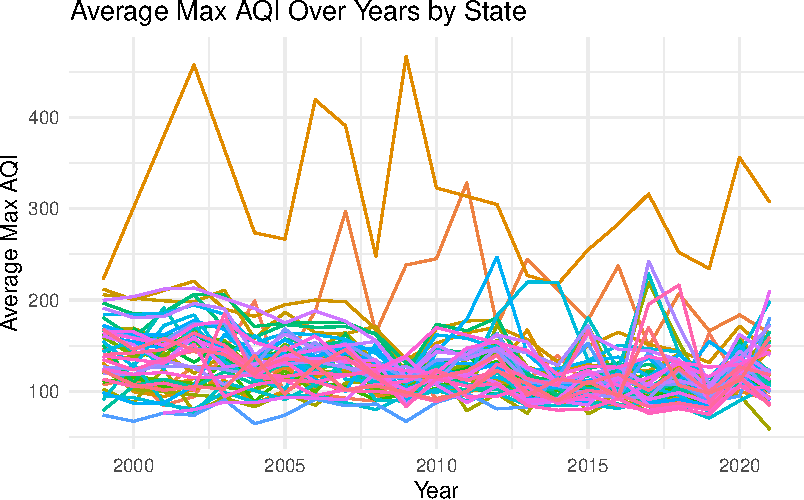
\includegraphics{final_main_quarto_presentation_files/figure-pdf/unnamed-chunk-4-1.pdf}

\begin{Shaded}
\begin{Highlighting}[]
\CommentTok{\# Average AQI by State}
\NormalTok{state\_avg\_aqi }\OtherTok{\textless{}{-}}\NormalTok{ cleaned\_data }\SpecialCharTok{\%\textgreater{}\%}
  \FunctionTok{group\_by}\NormalTok{(States) }\SpecialCharTok{\%\textgreater{}\%}
  \FunctionTok{summarise}\NormalTok{(}\AttributeTok{avg\_aqi =} \FunctionTok{mean}\NormalTok{(avg\_max\_aqi, }\AttributeTok{na.rm =} \ConstantTok{TRUE}\NormalTok{)) }\SpecialCharTok{\%\textgreater{}\%}
  \FunctionTok{arrange}\NormalTok{(}\FunctionTok{desc}\NormalTok{(avg\_aqi))}

\FunctionTok{ggplot}\NormalTok{(state\_avg\_aqi, }\FunctionTok{aes}\NormalTok{(}\AttributeTok{x =} \FunctionTok{reorder}\NormalTok{(States, avg\_aqi), }\AttributeTok{y =}\NormalTok{ avg\_aqi)) }\SpecialCharTok{+}
  \FunctionTok{geom\_bar}\NormalTok{(}\AttributeTok{stat =} \StringTok{"identity"}\NormalTok{, }\AttributeTok{fill =} \StringTok{"steelblue"}\NormalTok{) }\SpecialCharTok{+}
  \FunctionTok{coord\_flip}\NormalTok{() }\SpecialCharTok{+}
  \FunctionTok{theme\_minimal}\NormalTok{() }\SpecialCharTok{+}
  \FunctionTok{labs}\NormalTok{(}\AttributeTok{title =} \StringTok{"Average AQI by State"}\NormalTok{, }\AttributeTok{x =} \StringTok{"State"}\NormalTok{, }\AttributeTok{y =} \StringTok{"Average AQI"}\NormalTok{)}
\end{Highlighting}
\end{Shaded}

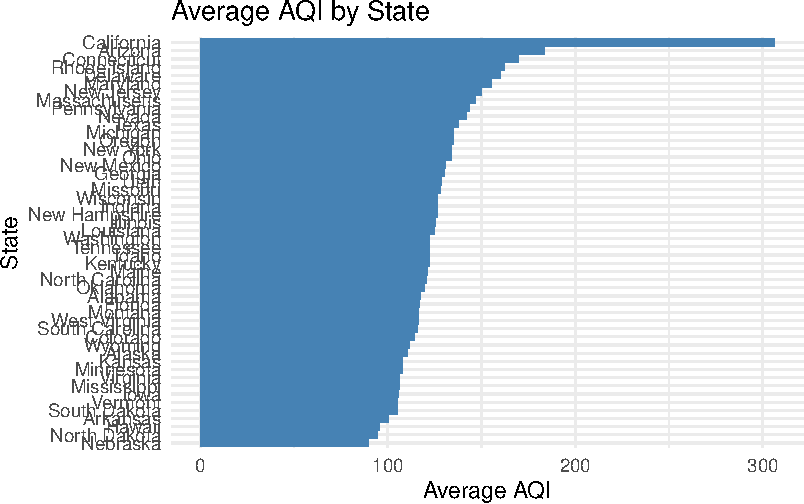
\includegraphics{final_main_quarto_presentation_files/figure-pdf/unnamed-chunk-5-1.pdf}

\begin{Shaded}
\begin{Highlighting}[]
\CommentTok{\# Scatter plot of AQI vs. Total Population}
\FunctionTok{ggplot}\NormalTok{(cleaned\_data, }\FunctionTok{aes}\NormalTok{(}\AttributeTok{x =}\NormalTok{ Total\_Population, }\AttributeTok{y =}\NormalTok{ avg\_max\_aqi)) }\SpecialCharTok{+}
  \FunctionTok{geom\_point}\NormalTok{(}\FunctionTok{aes}\NormalTok{(}\AttributeTok{color =}\NormalTok{ States), }\AttributeTok{alpha =} \FloatTok{0.6}\NormalTok{) }\SpecialCharTok{+}
  \FunctionTok{scale\_x\_continuous}\NormalTok{(}\AttributeTok{labels =}\NormalTok{ scales}\SpecialCharTok{::}\NormalTok{comma) }\SpecialCharTok{+}
  \FunctionTok{theme\_minimal}\NormalTok{() }\SpecialCharTok{+}
  \FunctionTok{labs}\NormalTok{(}\AttributeTok{title =} \StringTok{"Average AQI vs. Total Population"}\NormalTok{, }\AttributeTok{x =} \StringTok{"Total Population"}\NormalTok{, }\AttributeTok{y =} \StringTok{"Average AQI"}\NormalTok{)}
\end{Highlighting}
\end{Shaded}

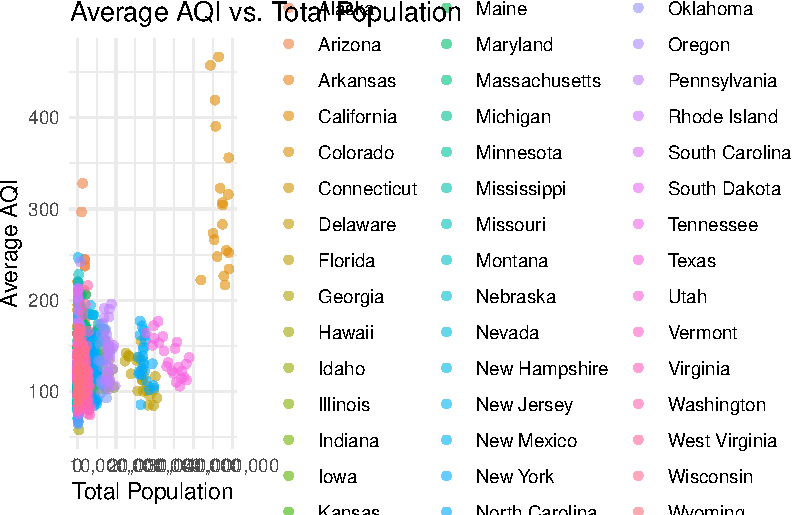
\includegraphics{final_main_quarto_presentation_files/figure-pdf/unnamed-chunk-6-1.pdf}

\begin{Shaded}
\begin{Highlighting}[]
\CommentTok{\# Histogram of the average maximum AQI}
\FunctionTok{ggplot}\NormalTok{(cleaned\_data, }\FunctionTok{aes}\NormalTok{(}\AttributeTok{x =}\NormalTok{ avg\_max\_aqi)) }\SpecialCharTok{+}
  \FunctionTok{geom\_histogram}\NormalTok{(}\AttributeTok{bins =} \DecValTok{30}\NormalTok{, }\AttributeTok{fill =} \StringTok{"dodgerblue"}\NormalTok{, }\AttributeTok{color =} \StringTok{"black"}\NormalTok{, }\AttributeTok{alpha =} \FloatTok{0.7}\NormalTok{) }\SpecialCharTok{+}
  \FunctionTok{theme\_minimal}\NormalTok{() }\SpecialCharTok{+}
  \FunctionTok{labs}\NormalTok{(}\AttributeTok{title =} \StringTok{"Distribution of Average Max AQI"}\NormalTok{, }\AttributeTok{x =} \StringTok{"Average Max AQI"}\NormalTok{, }\AttributeTok{y =} \StringTok{"Frequency"}\NormalTok{)}
\end{Highlighting}
\end{Shaded}

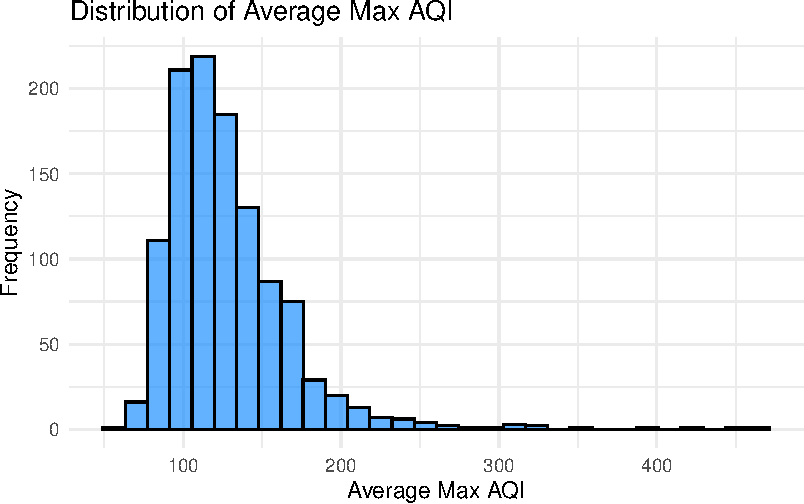
\includegraphics{final_main_quarto_presentation_files/figure-pdf/unnamed-chunk-7-1.pdf}

\begin{Shaded}
\begin{Highlighting}[]
\FunctionTok{library}\NormalTok{(ggplot2)}
\FunctionTok{library}\NormalTok{(dplyr)}

\CommentTok{\# Split states into two groups}
\NormalTok{state\_groups }\OtherTok{\textless{}{-}}\NormalTok{ cleaned\_data }\SpecialCharTok{\%\textgreater{}\%}
  \FunctionTok{mutate}\NormalTok{(}\AttributeTok{group =} \FunctionTok{ifelse}\NormalTok{(States }\SpecialCharTok{\%in\%} \FunctionTok{unique}\NormalTok{(States)[}\DecValTok{1}\SpecialCharTok{:}\DecValTok{25}\NormalTok{], }\StringTok{"Group 1"}\NormalTok{, }\StringTok{"Group 2"}\NormalTok{))}

\CommentTok{\# Function to create the plot for each group}
\NormalTok{create\_facet\_plot }\OtherTok{\textless{}{-}} \ControlFlowTok{function}\NormalTok{(data, title\_suffix) \{}
  \FunctionTok{ggplot}\NormalTok{(data, }\FunctionTok{aes}\NormalTok{(}\AttributeTok{x =}\NormalTok{ year, }\AttributeTok{y =}\NormalTok{ avg\_max\_aqi, }\AttributeTok{group =}\NormalTok{ States)) }\SpecialCharTok{+}
    \FunctionTok{geom\_line}\NormalTok{(}\AttributeTok{color =} \StringTok{"steelblue"}\NormalTok{, }\AttributeTok{size =} \FloatTok{0.8}\NormalTok{) }\SpecialCharTok{+}
    \FunctionTok{facet\_wrap}\NormalTok{(}\SpecialCharTok{\textasciitilde{}}\NormalTok{ States, }\AttributeTok{ncol =} \DecValTok{5}\NormalTok{, }\AttributeTok{nrow =} \DecValTok{5}\NormalTok{, }\AttributeTok{scales =} \StringTok{"free\_y"}\NormalTok{) }\SpecialCharTok{+}
    \FunctionTok{theme\_minimal}\NormalTok{(}\AttributeTok{base\_size =} \DecValTok{12}\NormalTok{) }\SpecialCharTok{+}
    \FunctionTok{labs}\NormalTok{(}
      \AttributeTok{title =} \FunctionTok{paste}\NormalTok{(}\StringTok{"State{-}Specific AQI Trends Over Years"}\NormalTok{, title\_suffix),}
      \AttributeTok{x =} \StringTok{"Year"}\NormalTok{, }\AttributeTok{y =} \StringTok{"Average Max AQI"}
\NormalTok{    ) }\SpecialCharTok{+}
    \FunctionTok{scale\_y\_continuous}\NormalTok{(}
      \AttributeTok{breaks =} \ControlFlowTok{function}\NormalTok{(x) }\FunctionTok{pretty}\NormalTok{(x, }\AttributeTok{n =} \DecValTok{3}\NormalTok{)}
\NormalTok{    ) }\SpecialCharTok{+}
    \FunctionTok{scale\_x\_continuous}\NormalTok{(}
      \AttributeTok{breaks =} \FunctionTok{seq}\NormalTok{(}
        \FunctionTok{min}\NormalTok{(cleaned\_data}\SpecialCharTok{$}\NormalTok{year, }\AttributeTok{na.rm =} \ConstantTok{TRUE}\NormalTok{),}
        \FunctionTok{max}\NormalTok{(cleaned\_data}\SpecialCharTok{$}\NormalTok{year, }\AttributeTok{na.rm =} \ConstantTok{TRUE}\NormalTok{),}
        \AttributeTok{by =} \DecValTok{5}
\NormalTok{      )}
\NormalTok{    ) }\SpecialCharTok{+}
    \FunctionTok{theme}\NormalTok{(}
      \AttributeTok{strip.text =} \FunctionTok{element\_text}\NormalTok{(}\AttributeTok{size =} \DecValTok{10}\NormalTok{, }\AttributeTok{face =} \StringTok{"bold"}\NormalTok{),}
      \AttributeTok{axis.text.x =} \FunctionTok{element\_text}\NormalTok{(}\AttributeTok{size =} \DecValTok{10}\NormalTok{, }\AttributeTok{angle =} \DecValTok{30}\NormalTok{, }\AttributeTok{hjust =} \DecValTok{1}\NormalTok{),}
      \AttributeTok{axis.text.y =} \FunctionTok{element\_text}\NormalTok{(}\AttributeTok{size =} \DecValTok{8}\NormalTok{),}
      \AttributeTok{plot.title =} \FunctionTok{element\_text}\NormalTok{(}\AttributeTok{size =} \DecValTok{16}\NormalTok{, }\AttributeTok{face =} \StringTok{"bold"}\NormalTok{),}
      \AttributeTok{panel.spacing =} \FunctionTok{unit}\NormalTok{(}\FloatTok{1.5}\NormalTok{, }\StringTok{"lines"}\NormalTok{),}
      \AttributeTok{plot.margin =} \FunctionTok{margin}\NormalTok{(}\DecValTok{10}\NormalTok{, }\DecValTok{10}\NormalTok{, }\DecValTok{10}\NormalTok{, }\DecValTok{10}\NormalTok{)}
\NormalTok{    )}
\NormalTok{\}}

\CommentTok{\# Generate plots for Group 1 and Group 2}
\NormalTok{plot\_group1 }\OtherTok{\textless{}{-}} \FunctionTok{create\_facet\_plot}\NormalTok{(state\_groups }\SpecialCharTok{\%\textgreater{}\%} \FunctionTok{filter}\NormalTok{(group }\SpecialCharTok{==} \StringTok{"Group 1"}\NormalTok{), }\StringTok{"(Group 1)"}\NormalTok{)}
\end{Highlighting}
\end{Shaded}

\begin{verbatim}
Warning: Using `size` aesthetic for lines was deprecated in ggplot2 3.4.0.
i Please use `linewidth` instead.
\end{verbatim}

\begin{Shaded}
\begin{Highlighting}[]
\NormalTok{plot\_group2 }\OtherTok{\textless{}{-}} \FunctionTok{create\_facet\_plot}\NormalTok{(state\_groups }\SpecialCharTok{\%\textgreater{}\%} \FunctionTok{filter}\NormalTok{(group }\SpecialCharTok{==} \StringTok{"Group 2"}\NormalTok{), }\StringTok{"(Group 2)"}\NormalTok{)}

\CommentTok{\# Save both plots to a single PDF}
\FunctionTok{pdf}\NormalTok{(}\StringTok{"state\_aqi\_trends\_split\_adjusted.pdf"}\NormalTok{, }\AttributeTok{width =} \DecValTok{18}\NormalTok{, }\AttributeTok{height =} \DecValTok{14}\NormalTok{)}

\FunctionTok{dev.off}\NormalTok{()}
\end{Highlighting}
\end{Shaded}

\begin{verbatim}
pdf 
  2 
\end{verbatim}

\begin{Shaded}
\begin{Highlighting}[]
\CommentTok{\# Density plot of unhealthy days}
\FunctionTok{ggplot}\NormalTok{(cleaned\_data, }\FunctionTok{aes}\NormalTok{(}\AttributeTok{x =}\NormalTok{ avg\_unhealthy\_days)) }\SpecialCharTok{+}
  \FunctionTok{geom\_density}\NormalTok{(}\AttributeTok{fill =} \StringTok{"lightblue"}\NormalTok{, }\AttributeTok{color =} \StringTok{"black"}\NormalTok{, }\AttributeTok{alpha =} \FloatTok{0.7}\NormalTok{) }\SpecialCharTok{+}
  \FunctionTok{theme\_minimal}\NormalTok{() }\SpecialCharTok{+}
  \FunctionTok{labs}\NormalTok{(}\AttributeTok{title =} \StringTok{"Density Plot of Unhealthy Days with AQI"}\NormalTok{, }
       \AttributeTok{x =} \StringTok{"Unhealthy Days"}\NormalTok{, }\AttributeTok{y =} \StringTok{"Density"}\NormalTok{)}
\end{Highlighting}
\end{Shaded}

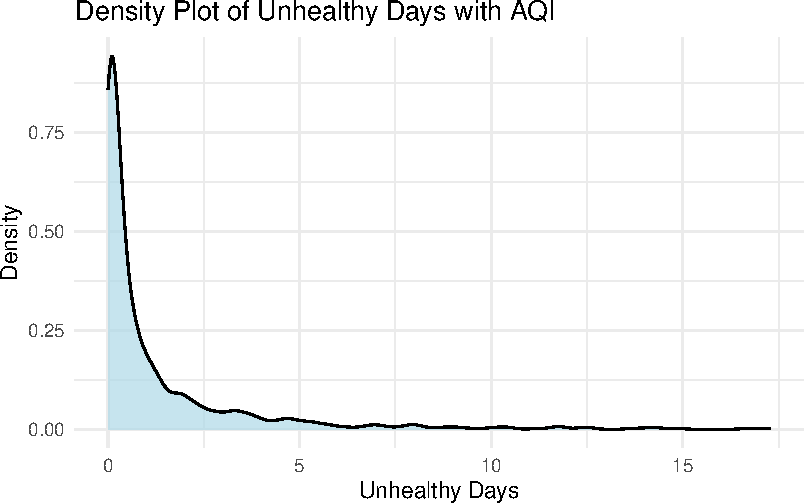
\includegraphics{final_main_quarto_presentation_files/figure-pdf/unnamed-chunk-9-1.pdf}

\begin{Shaded}
\begin{Highlighting}[]
\FunctionTok{library}\NormalTok{(ggplot2)}
\FunctionTok{library}\NormalTok{(dplyr)}

\CommentTok{\# Sort states by median unhealthy days}
\NormalTok{cleaned\_data }\OtherTok{\textless{}{-}}\NormalTok{ cleaned\_data }\SpecialCharTok{\%\textgreater{}\%}
  \FunctionTok{mutate}\NormalTok{(}\AttributeTok{States =} \FunctionTok{reorder}\NormalTok{(States, avg\_unhealthy\_days, median, }\AttributeTok{na.rm =} \ConstantTok{TRUE}\NormalTok{))}

\CommentTok{\# Create the boxplot with all 50 states}
\FunctionTok{ggplot}\NormalTok{(cleaned\_data, }\FunctionTok{aes}\NormalTok{(}\AttributeTok{x =}\NormalTok{ States, }\AttributeTok{y =}\NormalTok{ avg\_unhealthy\_days)) }\SpecialCharTok{+}
  \FunctionTok{geom\_boxplot}\NormalTok{(}\FunctionTok{aes}\NormalTok{(}\AttributeTok{fill =} \FunctionTok{as.factor}\NormalTok{(}\FunctionTok{cut}\NormalTok{(avg\_unhealthy\_days, }\AttributeTok{breaks =} \DecValTok{5}\NormalTok{))), }
               \AttributeTok{outlier.color =} \StringTok{"red"}\NormalTok{, }\AttributeTok{outlier.size =} \FloatTok{1.2}\NormalTok{) }\SpecialCharTok{+}
  \FunctionTok{scale\_fill\_manual}\NormalTok{(}\AttributeTok{values =} \FunctionTok{c}\NormalTok{(}\StringTok{"lightgreen"}\NormalTok{, }\StringTok{"darkgreen"}\NormalTok{, }\StringTok{"yellow"}\NormalTok{, }\StringTok{"orange"}\NormalTok{, }\StringTok{"red"}\NormalTok{)) }\SpecialCharTok{+}
  \FunctionTok{coord\_flip}\NormalTok{() }\SpecialCharTok{+}
  \FunctionTok{theme\_minimal}\NormalTok{(}\AttributeTok{base\_size =} \DecValTok{12}\NormalTok{) }\SpecialCharTok{+}
  \FunctionTok{labs}\NormalTok{(}
    \AttributeTok{title =} \StringTok{"Unhealthy AQI Days by State"}\NormalTok{,}
    \AttributeTok{x =} \StringTok{"State"}\NormalTok{,}
    \AttributeTok{y =} \StringTok{"Unhealthy Days"}\NormalTok{,}
    \AttributeTok{fill =} \StringTok{"Avg Unhealthy Days"}
\NormalTok{  ) }\SpecialCharTok{+}
  \FunctionTok{theme}\NormalTok{(}
    \AttributeTok{axis.text.y =} \FunctionTok{element\_text}\NormalTok{(}\AttributeTok{size =} \DecValTok{6}\NormalTok{, }\AttributeTok{vjust =} \DecValTok{1}\NormalTok{, }\AttributeTok{hjust =} \DecValTok{1}\NormalTok{),   }\CommentTok{\# Smaller y{-}axis text}
    \AttributeTok{axis.text.x =} \FunctionTok{element\_text}\NormalTok{(}\AttributeTok{size =} \DecValTok{10}\NormalTok{, }\AttributeTok{angle =} \DecValTok{90}\NormalTok{, }\AttributeTok{hjust =} \DecValTok{1}\NormalTok{),  }\CommentTok{\# Rotate x{-}axis labels}
    \AttributeTok{axis.ticks.y =} \FunctionTok{element\_blank}\NormalTok{(),}
    \AttributeTok{axis.title.x =} \FunctionTok{element\_text}\NormalTok{(}\AttributeTok{size =} \DecValTok{8}\NormalTok{),}
    \AttributeTok{axis.title.y =} \FunctionTok{element\_text}\NormalTok{(}\AttributeTok{size =} \DecValTok{8}\NormalTok{),}
    \AttributeTok{plot.title =} \FunctionTok{element\_text}\NormalTok{(}\AttributeTok{size =} \DecValTok{10}\NormalTok{, }\AttributeTok{face =} \StringTok{"bold"}\NormalTok{, }\AttributeTok{hjust =} \FloatTok{0.5}\NormalTok{),}
    \AttributeTok{legend.position =} \StringTok{"right"}\NormalTok{,}
    \AttributeTok{legend.key.width =} \FunctionTok{unit}\NormalTok{(}\DecValTok{1}\NormalTok{, }\StringTok{"cm"}\NormalTok{),}
    \AttributeTok{legend.title =} \FunctionTok{element\_text}\NormalTok{(}\AttributeTok{size =} \DecValTok{10}\NormalTok{),}
    \AttributeTok{legend.text =} \FunctionTok{element\_text}\NormalTok{(}\AttributeTok{size =} \DecValTok{10}\NormalTok{),}
    \AttributeTok{plot.margin =} \FunctionTok{margin}\NormalTok{(}\DecValTok{15}\NormalTok{, }\DecValTok{15}\NormalTok{, }\DecValTok{15}\NormalTok{, }\DecValTok{30}\NormalTok{),  }\CommentTok{\# Increased bottom margin for readability}
    \FunctionTok{scale\_y\_continuous}\NormalTok{(}\AttributeTok{breaks =} \FunctionTok{seq}\NormalTok{(}\DecValTok{0}\NormalTok{, }\FunctionTok{max}\NormalTok{(cleaned\_data}\SpecialCharTok{$}\NormalTok{avg\_unhealthy\_days), }\AttributeTok{by =} \DecValTok{2}\NormalTok{))}
\NormalTok{  )}
\end{Highlighting}
\end{Shaded}

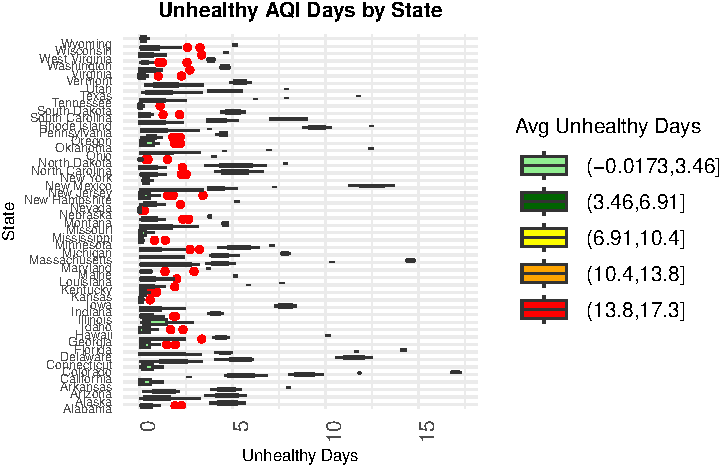
\includegraphics{final_main_quarto_presentation_files/figure-pdf/unnamed-chunk-10-1.pdf}

\begin{Shaded}
\begin{Highlighting}[]
\CommentTok{\# Ensure that the data is ungrouped}
\NormalTok{cleaned\_data }\OtherTok{\textless{}{-}}\NormalTok{ cleaned\_data }\SpecialCharTok{\%\textgreater{}\%} \FunctionTok{ungroup}\NormalTok{()}

\CommentTok{\# Select only numeric columns}
\NormalTok{numeric\_data }\OtherTok{\textless{}{-}}\NormalTok{ cleaned\_data }\SpecialCharTok{\%\textgreater{}\%}
  \FunctionTok{select}\NormalTok{(}\FunctionTok{where}\NormalTok{(is.numeric))}

\CommentTok{\# Compute the correlation matrix}
\NormalTok{cor\_matrix }\OtherTok{\textless{}{-}} \FunctionTok{cor}\NormalTok{(numeric\_data, }\AttributeTok{use =} \StringTok{"complete.obs"}\NormalTok{)}

\CommentTok{\# Print the correlation matrix}
\FunctionTok{print}\NormalTok{(cor\_matrix)}
\end{Highlighting}
\end{Shaded}

\begin{verbatim}
                                               year avg_max_aqi
year                                     1.00000000 -0.20389224
avg_max_aqi                             -0.20389224  1.00000000
avg_x90th_percentile_aqi                -0.40458365  0.67505568
avg_median_aqi                          -0.06242946  0.43023541
avg_days_with_aqi                        0.51328732  0.18689323
avg_good_days                            0.52834788 -0.21914710
avg_moderate_days                        0.07778249  0.41799183
avg_unhealthy_for_sensitive_groups_days -0.42288197  0.75389796
avg_unhealthy_days                      -0.32409289  0.69982723
avg_very_unhealthy_days                 -0.17403639  0.57327276
avg_hazardous_days                       0.04684586  0.47092206
avg_days_co                             -0.36038577  0.00597589
avg_days_no2                            -0.34590792  0.16998642
avg_days_ozone                           0.18421218  0.21403556
avg_days_pm2_5                           0.39884828 -0.07461222
avg_days_pm10                           -0.15157526 -0.02945708
Total_Count                              0.07464031  0.38499016
Total_Population                         0.05540930  0.42922529
                                        avg_x90th_percentile_aqi avg_median_aqi
year                                                 -0.40458365    -0.06242946
avg_max_aqi                                           0.67505568     0.43023541
avg_x90th_percentile_aqi                              1.00000000     0.76113660
avg_median_aqi                                        0.76113660     1.00000000
avg_days_with_aqi                                    -0.05852535     0.11039583
avg_good_days                                        -0.59264756    -0.49633038
avg_moderate_days                                     0.59505368     0.80730908
avg_unhealthy_for_sensitive_groups_days               0.89350965     0.55827852
avg_unhealthy_days                                    0.74726281     0.35560896
avg_very_unhealthy_days                               0.51590631     0.21966128
avg_hazardous_days                                    0.11984193     0.06503809
avg_days_co                                          -0.02286648    -0.28936071
avg_days_no2                                          0.22313611     0.00603191
avg_days_ozone                                        0.17467285     0.32324580
avg_days_pm2_5                                       -0.14944136    -0.01284501
avg_days_pm10                                        -0.23351251    -0.39672124
Total_Count                                           0.22642075     0.28137416
Total_Population                                      0.21154761     0.24237940
                                        avg_days_with_aqi avg_good_days
year                                          0.513287323    0.52834788
avg_max_aqi                                   0.186893225   -0.21914710
avg_x90th_percentile_aqi                     -0.058525354   -0.59264756
avg_median_aqi                                0.110395831   -0.49633038
avg_days_with_aqi                             1.000000000    0.73257772
avg_good_days                                 0.732577720    1.00000000
avg_moderate_days                             0.394388796   -0.31929829
avg_unhealthy_for_sensitive_groups_days       0.000625128   -0.45940877
avg_unhealthy_days                            0.028316496   -0.28844662
avg_very_unhealthy_days                       0.083733620   -0.13114912
avg_hazardous_days                            0.093843201   -0.02179993
avg_days_co                                  -0.235611637   -0.09603969
avg_days_no2                                 -0.055856650   -0.07456027
avg_days_ozone                                0.459928593    0.33271019
avg_days_pm2_5                                0.439230933    0.25497011
avg_days_pm10                                -0.136254178    0.06622098
Total_Count                                   0.352872423    0.07688920
Total_Population                              0.334413071    0.07869097
                                        avg_moderate_days
year                                           0.07778249
avg_max_aqi                                    0.41799183
avg_x90th_percentile_aqi                       0.59505368
avg_median_aqi                                 0.80730908
avg_days_with_aqi                              0.39438880
avg_good_days                                 -0.31929829
avg_moderate_days                              1.00000000
avg_unhealthy_for_sensitive_groups_days        0.45018608
avg_unhealthy_days                             0.24722668
avg_very_unhealthy_days                        0.15510053
avg_hazardous_days                             0.10821568
avg_days_co                                   -0.23376351
avg_days_no2                                  -0.05531032
avg_days_ozone                                 0.13492094
avg_days_pm2_5                                 0.33928718
avg_days_pm10                                 -0.29800418
Total_Count                                    0.34048722
Total_Population                               0.30168383
                                        avg_unhealthy_for_sensitive_groups_days
year                                                               -0.422881975
avg_max_aqi                                                         0.753897962
avg_x90th_percentile_aqi                                            0.893509646
avg_median_aqi                                                      0.558278521
avg_days_with_aqi                                                   0.000625128
avg_good_days                                                      -0.459408772
avg_moderate_days                                                   0.450186081
avg_unhealthy_for_sensitive_groups_days                             1.000000000
avg_unhealthy_days                                                  0.805958249
avg_very_unhealthy_days                                             0.534647716
avg_hazardous_days                                                  0.227486772
avg_days_co                                                         0.059916787
avg_days_no2                                                        0.299907536
avg_days_ozone                                                      0.218194126
avg_days_pm2_5                                                     -0.240317292
avg_days_pm10                                                      -0.059633416
Total_Count                                                         0.302518082
Total_Population                                                    0.322974733
                                        avg_unhealthy_days
year                                           -0.32409289
avg_max_aqi                                     0.69982723
avg_x90th_percentile_aqi                        0.74726281
avg_median_aqi                                  0.35560896
avg_days_with_aqi                               0.02831650
avg_good_days                                  -0.28844662
avg_moderate_days                               0.24722668
avg_unhealthy_for_sensitive_groups_days         0.80595825
avg_unhealthy_days                              1.00000000
avg_very_unhealthy_days                         0.76964250
avg_hazardous_days                              0.21921110
avg_days_co                                     0.08807261
avg_days_no2                                    0.29527107
avg_days_ozone                                  0.11344716
avg_days_pm2_5                                 -0.11371631
avg_days_pm10                                  -0.09166169
Total_Count                                     0.27606581
Total_Population                                0.31169762
                                        avg_very_unhealthy_days
year                                                -0.17403639
avg_max_aqi                                          0.57327276
avg_x90th_percentile_aqi                             0.51590631
avg_median_aqi                                       0.21966128
avg_days_with_aqi                                    0.08373362
avg_good_days                                       -0.13114912
avg_moderate_days                                    0.15510053
avg_unhealthy_for_sensitive_groups_days              0.53464772
avg_unhealthy_days                                   0.76964250
avg_very_unhealthy_days                              1.00000000
avg_hazardous_days                                   0.29490230
avg_days_co                                          0.06964201
avg_days_no2                                         0.21232792
avg_days_ozone                                       0.09863070
avg_days_pm2_5                                      -0.08387798
avg_days_pm10                                        0.01785630
Total_Count                                          0.17874893
Total_Population                                     0.20704068
                                        avg_hazardous_days avg_days_co
year                                            0.04684586 -0.36038577
avg_max_aqi                                     0.47092206  0.00597589
avg_x90th_percentile_aqi                        0.11984193 -0.02286648
avg_median_aqi                                  0.06503809 -0.28936071
avg_days_with_aqi                               0.09384320 -0.23561164
avg_good_days                                  -0.02179993 -0.09603969
avg_moderate_days                               0.10821568 -0.23376351
avg_unhealthy_for_sensitive_groups_days         0.22748677  0.05991679
avg_unhealthy_days                              0.21921110  0.08807261
avg_very_unhealthy_days                         0.29490230  0.06964201
avg_hazardous_days                              1.00000000 -0.02986652
avg_days_co                                    -0.02986652  1.00000000
avg_days_no2                                   -0.04849440  0.21806297
avg_days_ozone                                  0.04093125 -0.25727199
avg_days_pm2_5                                 -0.06949123 -0.21643031
avg_days_pm10                                   0.28832028  0.24549284
Total_Count                                     0.15173717 -0.04779091
Total_Population                                0.18732776 -0.05119970
                                        avg_days_no2 avg_days_ozone
year                                     -0.34590792     0.18421218
avg_max_aqi                               0.16998642     0.21403556
avg_x90th_percentile_aqi                  0.22313611     0.17467285
avg_median_aqi                            0.00603191     0.32324580
avg_days_with_aqi                        -0.05585665     0.45992859
avg_good_days                            -0.07456027     0.33271019
avg_moderate_days                        -0.05531032     0.13492094
avg_unhealthy_for_sensitive_groups_days   0.29990754     0.21819413
avg_unhealthy_days                        0.29527107     0.11344716
avg_very_unhealthy_days                   0.21232792     0.09863070
avg_hazardous_days                       -0.04849440     0.04093125
avg_days_co                               0.21806297    -0.25727199
avg_days_no2                              1.00000000     0.05359207
avg_days_ozone                            0.05359207     1.00000000
avg_days_pm2_5                           -0.27828246    -0.47238543
avg_days_pm10                            -0.09209680    -0.15857884
Total_Count                               0.04576440     0.29381918
Total_Population                          0.03387115     0.27599105
                                        avg_days_pm2_5 avg_days_pm10
year                                        0.39884828   -0.15157526
avg_max_aqi                                -0.07461222   -0.02945708
avg_x90th_percentile_aqi                   -0.14944136   -0.23351251
avg_median_aqi                             -0.01284501   -0.39672124
avg_days_with_aqi                           0.43923093   -0.13625418
avg_good_days                               0.25497011    0.06622098
avg_moderate_days                           0.33928718   -0.29800418
avg_unhealthy_for_sensitive_groups_days    -0.24031729   -0.05963342
avg_unhealthy_days                         -0.11371631   -0.09166169
avg_very_unhealthy_days                    -0.08387798    0.01785630
avg_hazardous_days                         -0.06949123    0.28832028
avg_days_co                                -0.21643031    0.24549284
avg_days_no2                               -0.27828246   -0.09209680
avg_days_ozone                             -0.47238543   -0.15857884
avg_days_pm2_5                              1.00000000   -0.37890019
avg_days_pm10                              -0.37890019    1.00000000
Total_Count                                 0.08251445   -0.20700995
Total_Population                            0.06996585   -0.16392800
                                        Total_Count Total_Population
year                                     0.07464031       0.05540930
avg_max_aqi                              0.38499016       0.42922529
avg_x90th_percentile_aqi                 0.22642075       0.21154761
avg_median_aqi                           0.28137416       0.24237940
avg_days_with_aqi                        0.35287242       0.33441307
avg_good_days                            0.07688920       0.07869097
avg_moderate_days                        0.34048722       0.30168383
avg_unhealthy_for_sensitive_groups_days  0.30251808       0.32297473
avg_unhealthy_days                       0.27606581       0.31169762
avg_very_unhealthy_days                  0.17874893       0.20704068
avg_hazardous_days                       0.15173717       0.18732776
avg_days_co                             -0.04779091      -0.05119970
avg_days_no2                             0.04576440       0.03387115
avg_days_ozone                           0.29381918       0.27599105
avg_days_pm2_5                           0.08251445       0.06996585
avg_days_pm10                           -0.20700995      -0.16392800
Total_Count                              1.00000000       0.97170413
Total_Population                         0.97170413       1.00000000
\end{verbatim}

\begin{Shaded}
\begin{Highlighting}[]
\CommentTok{\# Visualize the correlation matrix using a heatmap}
\FunctionTok{heatmap}\NormalTok{(cor\_matrix, }
        \AttributeTok{main =} \StringTok{"Correlation Matrix"}\NormalTok{, }
        \AttributeTok{col =} \FunctionTok{colorRampPalette}\NormalTok{(}\FunctionTok{c}\NormalTok{(}\StringTok{"blue"}\NormalTok{, }\StringTok{"white"}\NormalTok{, }\StringTok{"red"}\NormalTok{))(}\DecValTok{100}\NormalTok{), }
        \AttributeTok{scale =} \StringTok{"none"}\NormalTok{, }
        \AttributeTok{margins =} \FunctionTok{c}\NormalTok{(}\DecValTok{8}\NormalTok{, }\DecValTok{8}\NormalTok{))}
\end{Highlighting}
\end{Shaded}

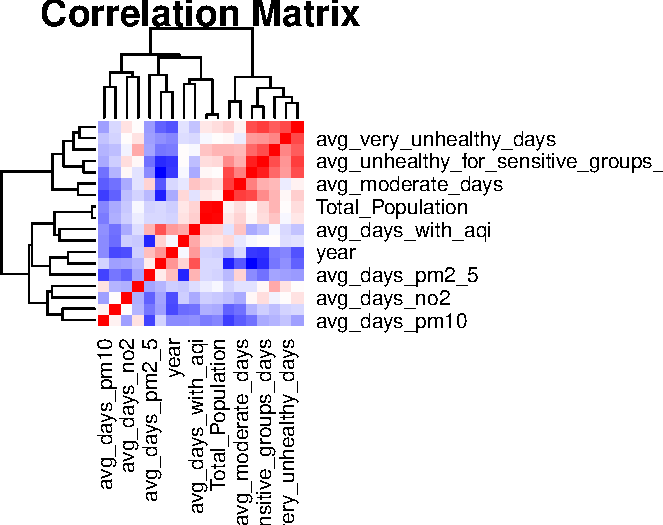
\includegraphics{final_main_quarto_presentation_files/figure-pdf/unnamed-chunk-11-1.pdf}

\begin{Shaded}
\begin{Highlighting}[]
\CommentTok{\# Selecting relevant numeric columns for correlation}
\NormalTok{correlation\_data }\OtherTok{\textless{}{-}}\NormalTok{ cleaned\_data }\SpecialCharTok{\%\textgreater{}\%}
  \FunctionTok{select}\NormalTok{(Total\_Count, avg\_max\_aqi, avg\_moderate\_days, avg\_unhealthy\_days, avg\_very\_unhealthy\_days, avg\_days\_pm2\_5)}

\CommentTok{\# Calculating correlation matrix for selected variables}
\NormalTok{cor\_matrix }\OtherTok{\textless{}{-}} \FunctionTok{cor}\NormalTok{(correlation\_data, }\AttributeTok{use =} \StringTok{"complete.obs"}\NormalTok{)}

\CommentTok{\# Viewing the correlation matrix}
\FunctionTok{print}\NormalTok{(cor\_matrix)}
\end{Highlighting}
\end{Shaded}

\begin{verbatim}
                        Total_Count avg_max_aqi avg_moderate_days
Total_Count              1.00000000  0.38499016         0.3404872
avg_max_aqi              0.38499016  1.00000000         0.4179918
avg_moderate_days        0.34048722  0.41799183         1.0000000
avg_unhealthy_days       0.27606581  0.69982723         0.2472267
avg_very_unhealthy_days  0.17874893  0.57327276         0.1551005
avg_days_pm2_5           0.08251445 -0.07461222         0.3392872
                        avg_unhealthy_days avg_very_unhealthy_days
Total_Count                      0.2760658              0.17874893
avg_max_aqi                      0.6998272              0.57327276
avg_moderate_days                0.2472267              0.15510053
avg_unhealthy_days               1.0000000              0.76964250
avg_very_unhealthy_days          0.7696425              1.00000000
avg_days_pm2_5                  -0.1137163             -0.08387798
                        avg_days_pm2_5
Total_Count                 0.08251445
avg_max_aqi                -0.07461222
avg_moderate_days           0.33928718
avg_unhealthy_days         -0.11371631
avg_very_unhealthy_days    -0.08387798
avg_days_pm2_5              1.00000000
\end{verbatim}

\begin{Shaded}
\begin{Highlighting}[]
\CommentTok{\# Summing Total\_Count across all states by year}
\NormalTok{total\_cancer\_by\_year }\OtherTok{\textless{}{-}}\NormalTok{ cleaned\_data }\SpecialCharTok{\%\textgreater{}\%}
  \FunctionTok{group\_by}\NormalTok{(year) }\SpecialCharTok{\%\textgreater{}\%}
  \FunctionTok{summarise}\NormalTok{(}\AttributeTok{total\_cancer\_incidence =} \FunctionTok{sum}\NormalTok{(Total\_Count, }\AttributeTok{na.rm =} \ConstantTok{TRUE}\NormalTok{), }\AttributeTok{.groups =} \StringTok{"drop"}\NormalTok{)}

\CommentTok{\# Plotting cancer incidence over time}
\FunctionTok{ggplot}\NormalTok{(total\_cancer\_by\_year, }\FunctionTok{aes}\NormalTok{(}\AttributeTok{x =}\NormalTok{ year, }\AttributeTok{y =}\NormalTok{ total\_cancer\_incidence)) }\SpecialCharTok{+}
  \FunctionTok{geom\_line}\NormalTok{(}\AttributeTok{color =} \StringTok{"blue"}\NormalTok{) }\SpecialCharTok{+}
  \FunctionTok{geom\_point}\NormalTok{(}\AttributeTok{color =} \StringTok{"red"}\NormalTok{) }\SpecialCharTok{+}
  \FunctionTok{labs}\NormalTok{(}\AttributeTok{title =} \StringTok{"Total Cancer Incidence Over Time (All States)"}\NormalTok{, }
       \AttributeTok{x =} \StringTok{"Year"}\NormalTok{, }
       \AttributeTok{y =} \StringTok{"Total Cancer Incidence"}\NormalTok{) }\SpecialCharTok{+}
  \FunctionTok{theme\_minimal}\NormalTok{()}
\end{Highlighting}
\end{Shaded}

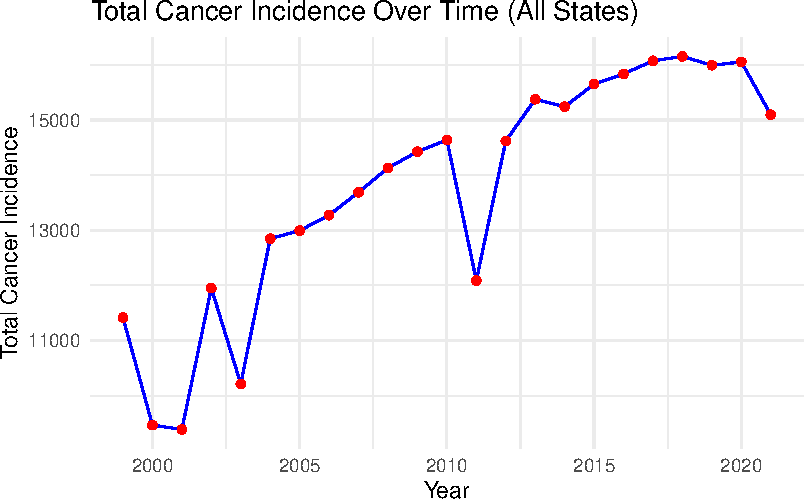
\includegraphics{final_main_quarto_presentation_files/figure-pdf/unnamed-chunk-13-1.pdf}

\begin{Shaded}
\begin{Highlighting}[]
\CommentTok{\# Summarizing Total\_Count by State}
\NormalTok{state\_summary }\OtherTok{\textless{}{-}}\NormalTok{ cleaned\_data }\SpecialCharTok{\%\textgreater{}\%}
  \FunctionTok{group\_by}\NormalTok{(States) }\SpecialCharTok{\%\textgreater{}\%}
  \FunctionTok{summarise}\NormalTok{(}
    \AttributeTok{avg\_total\_count =} \FunctionTok{mean}\NormalTok{(Total\_Count, }\AttributeTok{na.rm =} \ConstantTok{TRUE}\NormalTok{),}
    \AttributeTok{total\_total\_count =} \FunctionTok{sum}\NormalTok{(Total\_Count, }\AttributeTok{na.rm =} \ConstantTok{TRUE}\NormalTok{),}
    \AttributeTok{.groups =} \StringTok{"drop"}
\NormalTok{  )}

\CommentTok{\# Viewing the summarized data}
\FunctionTok{head}\NormalTok{(state\_summary)}
\end{Highlighting}
\end{Shaded}

\begin{verbatim}
# A tibble: 6 x 3
  States     avg_total_count total_total_count
  <fct>                <dbl>             <dbl>
1 Alabama              123                2829
2 Alaska                 0                   0
3 Arizona              221.               5076
4 Arkansas              20.3               447
5 California          2300.              43705
6 Colorado             108.               2489
\end{verbatim}

\begin{Shaded}
\begin{Highlighting}[]
\CommentTok{\# Calculating total cancer incidence and total population by state}
\NormalTok{state\_proportion }\OtherTok{\textless{}{-}}\NormalTok{ cleaned\_data }\SpecialCharTok{\%\textgreater{}\%}
  \FunctionTok{group\_by}\NormalTok{(States) }\SpecialCharTok{\%\textgreater{}\%}
  \FunctionTok{summarise}\NormalTok{(}
    \AttributeTok{total\_cancer =} \FunctionTok{sum}\NormalTok{(Total\_Count, }\AttributeTok{na.rm =} \ConstantTok{TRUE}\NormalTok{),}
    \AttributeTok{total\_population =} \FunctionTok{sum}\NormalTok{(Total\_Population, }\AttributeTok{na.rm =} \ConstantTok{TRUE}\NormalTok{),}
    \AttributeTok{cancer\_proportion =}\NormalTok{ total\_cancer }\SpecialCharTok{/}\NormalTok{ total\_population,}
    \AttributeTok{.groups =} \StringTok{"drop"}
\NormalTok{  )}

\CommentTok{\# Plotting the cancer incidence proportion by state}
\FunctionTok{ggplot}\NormalTok{(state\_proportion, }\FunctionTok{aes}\NormalTok{(}\AttributeTok{x =} \FunctionTok{reorder}\NormalTok{(States, cancer\_proportion), }\AttributeTok{y =}\NormalTok{ cancer\_proportion)) }\SpecialCharTok{+}
  \FunctionTok{geom\_bar}\NormalTok{(}\AttributeTok{stat =} \StringTok{"identity"}\NormalTok{, }\AttributeTok{fill =} \StringTok{"lightblue"}\NormalTok{) }\SpecialCharTok{+}
  \FunctionTok{coord\_flip}\NormalTok{() }\SpecialCharTok{+}
  \FunctionTok{labs}\NormalTok{(}\AttributeTok{title =} \StringTok{"Cancer Incidence as Proportion of Population by State"}\NormalTok{, }
       \AttributeTok{x =} \StringTok{"State"}\NormalTok{, }
       \AttributeTok{y =} \StringTok{"Cancer Incidence Proportion"}\NormalTok{) }\SpecialCharTok{+}
  \FunctionTok{theme\_minimal}\NormalTok{()}
\end{Highlighting}
\end{Shaded}

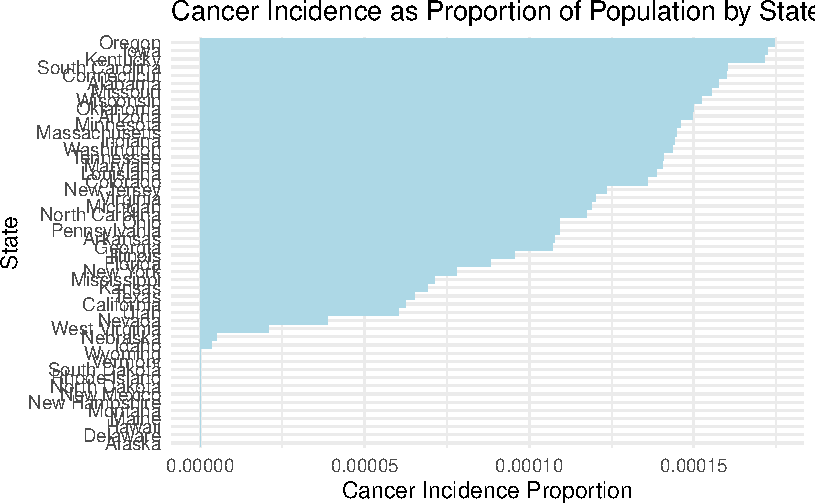
\includegraphics{final_main_quarto_presentation_files/figure-pdf/unnamed-chunk-15-1.pdf}

we specify the following priors:

\begin{itemize}
\item
  \(α\) \textasciitilde{} Normal(0, 10): The prior for the intercept is
  a normal distribution with a mean of 0 and a large standard deviation
  of 10, reflecting uncertainty about the baseline incidence.
\item
  \(β_k\) \textasciitilde{} Normal(0, 10) for each element β\_k: The
  priors for the coefficients of the predictors are also normally
  distributed with mean 0 and a large standard deviation of 10, allowing
  for flexibility in how predictors affect the cancer incidence count.
\item
  \(λ\) \textasciitilde{} Gamma(2, 0.1): This is the prior for the rate
  parameter in the Poisson distribution, with a mean of 2 and a large
  variance, allowing the model to adapt to the observed data.
\end{itemize}

These priors are relatively weak, meaning that they do not overly
constrain the model. They are designed to allow the data to drive the
inference

\begin{Shaded}
\begin{Highlighting}[]
\CommentTok{\# Define the predictors and response variable}
\NormalTok{predictors }\OtherTok{\textless{}{-}} \FunctionTok{c}\NormalTok{(}\StringTok{"avg\_max\_aqi"}\NormalTok{, }\StringTok{"avg\_moderate\_days"}\NormalTok{, }\StringTok{"avg\_unhealthy\_days"}\NormalTok{, }\StringTok{"avg\_very\_unhealthy\_days"}\NormalTok{, }\StringTok{"avg\_days\_pm2\_5"}\NormalTok{)}
\NormalTok{response }\OtherTok{\textless{}{-}} \StringTok{"Total\_Count"}

\CommentTok{\# Subset the data for predictors and response}
\NormalTok{data\_for\_model }\OtherTok{\textless{}{-}}\NormalTok{ cleaned\_data }\SpecialCharTok{\%\textgreater{}\%}
  \FunctionTok{select}\NormalTok{(States, year, }\FunctionTok{all\_of}\NormalTok{(predictors), response) }\SpecialCharTok{\%\textgreater{}\%}
  \FunctionTok{na.omit}\NormalTok{()}
\end{Highlighting}
\end{Shaded}

\begin{verbatim}
Warning: Using an external vector in selections was deprecated in tidyselect 1.1.0.
i Please use `all_of()` or `any_of()` instead.
  # Was:
  data %>% select(response)

  # Now:
  data %>% select(all_of(response))

See <https://tidyselect.r-lib.org/reference/faq-external-vector.html>.
\end{verbatim}

\begin{Shaded}
\begin{Highlighting}[]
\CommentTok{\# Create a matrix for predictors (X) and a vector for the response (y)}
\NormalTok{X }\OtherTok{\textless{}{-}} \FunctionTok{as.matrix}\NormalTok{(data\_for\_model[, predictors])}
\NormalTok{y }\OtherTok{\textless{}{-}}\NormalTok{ data\_for\_model[, response]}

\CommentTok{\# Define the number of observations (N), time periods (T), and predictors (K)}
\NormalTok{N }\OtherTok{\textless{}{-}} \FunctionTok{nrow}\NormalTok{(X)}
\NormalTok{T }\OtherTok{\textless{}{-}} \FunctionTok{length}\NormalTok{(}\FunctionTok{unique}\NormalTok{(data\_for\_model}\SpecialCharTok{$}\NormalTok{year))}
\NormalTok{K }\OtherTok{\textless{}{-}} \FunctionTok{ncol}\NormalTok{(X)}
\end{Highlighting}
\end{Shaded}

The likelihood of the data is specified as a Poisson distribution, where
the observed total cancer count \(y_i\) for each state-year pair follows
a Poisson distribution with parameter \(λ_i\)

The rate \(λ_i\) is the exponential of a linear combination of the
predictors. This captures the multiplicative effects of the predictors
on the expected cancer incidence.

\begin{Shaded}
\begin{Highlighting}[]
\CommentTok{\# Prepare the data list for STAN}
\NormalTok{stan\_data }\OtherTok{\textless{}{-}} \FunctionTok{list}\NormalTok{(}
  \AttributeTok{N =}\NormalTok{ N,}
  \AttributeTok{T =}\NormalTok{ T,}
  \AttributeTok{K =}\NormalTok{ K,}
  \AttributeTok{X =}\NormalTok{ X,}
  \AttributeTok{y =}\NormalTok{ y}
\NormalTok{)}
\end{Highlighting}
\end{Shaded}

The posterior distribution is the updated belief about the parameters
after observing the data. It is obtained by applying Bayes' theorem:

\(P(α, β | y, X) ∝ P(y | X, α, β) * P(α) * P(β)\)\\
Where:

\begin{itemize}
\item
  \(P(y | X, α, β)\) is the likelihood, as specified above.
\item
  \(P(α)\) and \(P(β)\) are the priors for the parameters \(α\) and
  \(β\).
\item
  The posterior distribution reflects the parameter estimates that are
  most consistent with the observed data, while also incorporating prior
  beliefs.
\end{itemize}

\begin{Shaded}
\begin{Highlighting}[]
\FunctionTok{library}\NormalTok{(rstan)}
\end{Highlighting}
\end{Shaded}

\begin{verbatim}
Loading required package: StanHeaders
\end{verbatim}

\begin{verbatim}

rstan version 2.32.6 (Stan version 2.32.2)
\end{verbatim}

\begin{verbatim}
For execution on a local, multicore CPU with excess RAM we recommend calling
options(mc.cores = parallel::detectCores()).
To avoid recompilation of unchanged Stan programs, we recommend calling
rstan_options(auto_write = TRUE)
For within-chain threading using `reduce_sum()` or `map_rect()` Stan functions,
change `threads_per_chain` option:
rstan_options(threads_per_chain = 1)
\end{verbatim}

\begin{verbatim}
Do not specify '-march=native' in 'LOCAL_CPPFLAGS' or a Makevars file
\end{verbatim}

\begin{verbatim}

Attaching package: 'rstan'
\end{verbatim}

\begin{verbatim}
The following object is masked from 'package:tidyr':

    extract
\end{verbatim}

\begin{Shaded}
\begin{Highlighting}[]
\FunctionTok{rstan\_options}\NormalTok{(}\AttributeTok{auto\_write =} \ConstantTok{TRUE}\NormalTok{)}
\FunctionTok{options}\NormalTok{(}\AttributeTok{mc.cores =}\NormalTok{ parallel}\SpecialCharTok{::}\FunctionTok{detectCores}\NormalTok{())}

\NormalTok{model }\OtherTok{\textless{}{-}} \FunctionTok{stan\_model}\NormalTok{(}\StringTok{"finalmodel.stan"}\NormalTok{)}

\NormalTok{y }\OtherTok{\textless{}{-}} \FunctionTok{as.vector}\NormalTok{(cleaned\_data}\SpecialCharTok{$}\NormalTok{Total\_Count)}
\NormalTok{N }\OtherTok{\textless{}{-}} \FunctionTok{length}\NormalTok{(y)}

\NormalTok{state\_levels }\OtherTok{\textless{}{-}} \FunctionTok{unique}\NormalTok{(cleaned\_data}\SpecialCharTok{$}\NormalTok{States)}
\NormalTok{state\_index }\OtherTok{\textless{}{-}} \FunctionTok{as.integer}\NormalTok{(}\FunctionTok{factor}\NormalTok{(cleaned\_data}\SpecialCharTok{$}\NormalTok{States, }\AttributeTok{levels =}\NormalTok{ state\_levels))}

\NormalTok{year\_index }\OtherTok{\textless{}{-}}\NormalTok{ cleaned\_data}\SpecialCharTok{$}\NormalTok{year}
\NormalTok{X }\OtherTok{\textless{}{-}}\NormalTok{ cleaned\_data[, }\FunctionTok{c}\NormalTok{(}\StringTok{"avg\_max\_aqi"}\NormalTok{, }\StringTok{"avg\_days\_with\_aqi"}\NormalTok{, }\StringTok{"avg\_good\_days"}\NormalTok{, }
                      \StringTok{"avg\_moderate\_days"}\NormalTok{, }\StringTok{"avg\_unhealthy\_days"}\NormalTok{)]}

\NormalTok{stan\_data }\OtherTok{\textless{}{-}} \FunctionTok{list}\NormalTok{(}
  \AttributeTok{N =}\NormalTok{ N,}
  \AttributeTok{K =} \FunctionTok{ncol}\NormalTok{(X),}
  \AttributeTok{y =}\NormalTok{ y,}
  \AttributeTok{X =}\NormalTok{ X,}
  \AttributeTok{state\_index =}\NormalTok{ state\_index,}
  \AttributeTok{year\_index =}\NormalTok{ year\_index,}
  \AttributeTok{S =} \FunctionTok{length}\NormalTok{(state\_levels)}
\NormalTok{)}

\NormalTok{fit }\OtherTok{\textless{}{-}} \FunctionTok{sampling}\NormalTok{(model, }\AttributeTok{data =}\NormalTok{ stan\_data, }\AttributeTok{iter =} \DecValTok{4000}\NormalTok{, }\AttributeTok{chains =} \DecValTok{4}\NormalTok{)}
\end{Highlighting}
\end{Shaded}

\begin{verbatim}
Warning: There were 5 divergent transitions after warmup. See
https://mc-stan.org/misc/warnings.html#divergent-transitions-after-warmup
to find out why this is a problem and how to eliminate them.
\end{verbatim}

\begin{verbatim}
Warning: There were 41 transitions after warmup that exceeded the maximum treedepth. Increase max_treedepth above 10. See
https://mc-stan.org/misc/warnings.html#maximum-treedepth-exceeded
\end{verbatim}

\begin{verbatim}
Warning: There were 3 chains where the estimated Bayesian Fraction of Missing Information was low. See
https://mc-stan.org/misc/warnings.html#bfmi-low
\end{verbatim}

\begin{verbatim}
Warning: Examine the pairs() plot to diagnose sampling problems
\end{verbatim}

\begin{verbatim}
Warning: The largest R-hat is 5.74, indicating chains have not mixed.
Running the chains for more iterations may help. See
https://mc-stan.org/misc/warnings.html#r-hat
\end{verbatim}

\begin{verbatim}
Warning: Bulk Effective Samples Size (ESS) is too low, indicating posterior means and medians may be unreliable.
Running the chains for more iterations may help. See
https://mc-stan.org/misc/warnings.html#bulk-ess
\end{verbatim}

\begin{verbatim}
Warning: Tail Effective Samples Size (ESS) is too low, indicating posterior variances and tail quantiles may be unreliable.
Running the chains for more iterations may help. See
https://mc-stan.org/misc/warnings.html#tail-ess
\end{verbatim}

\begin{Shaded}
\begin{Highlighting}[]
\FunctionTok{print}\NormalTok{(fit)}
\end{Highlighting}
\end{Shaded}

\begin{verbatim}
Inference for Stan model: anon_model.
4 chains, each with iter=4000; warmup=2000; thin=1; 
post-warmup draws per chain=2000, total post-warmup draws=8000.

         mean se_mean   sd  2.5%   25%        50%       75%      97.5% n_eff
alpha    0.42    1.06 1.50 -1.52 -0.81       0.60      1.82       1.98     2
beta[1] -0.39    0.52 0.74 -1.67 -0.86       0.01      0.06       0.07     2
beta[2] -0.58    0.41 0.60 -1.19 -0.96      -0.82      0.23       0.51     2
beta[3]  0.20    0.54 0.77 -0.69 -0.56      -0.25      0.95       1.17     2
beta[4]  0.24    0.54 0.79 -0.60 -0.58      -0.26      0.99       1.23     2
beta[5] -0.49    0.73 1.03 -1.58 -1.24      -0.81      0.21       1.14     2
lambda   1.09    0.58 0.81  0.16  0.37       1.03      1.75       2.12     2
lp__     -Inf     NaN  NaN  -Inf  -Inf -129962.95 906841.78 1148636.44   NaN
           Rhat
alpha   4078.50
beta[1]   28.79
beta[2]    7.57
beta[3]   10.37
beta[4]    8.19
beta[5]   52.03
lambda  1728.70
lp__        NaN

Samples were drawn using NUTS(diag_e) at Thu Dec 19 06:05:12 2024.
For each parameter, n_eff is a crude measure of effective sample size,
and Rhat is the potential scale reduction factor on split chains (at 
convergence, Rhat=1).
\end{verbatim}

\begin{Shaded}
\begin{Highlighting}[]
\NormalTok{samples }\OtherTok{\textless{}{-}} \FunctionTok{extract}\NormalTok{(fit)}

\FunctionTok{traceplot}\NormalTok{(fit)}
\end{Highlighting}
\end{Shaded}

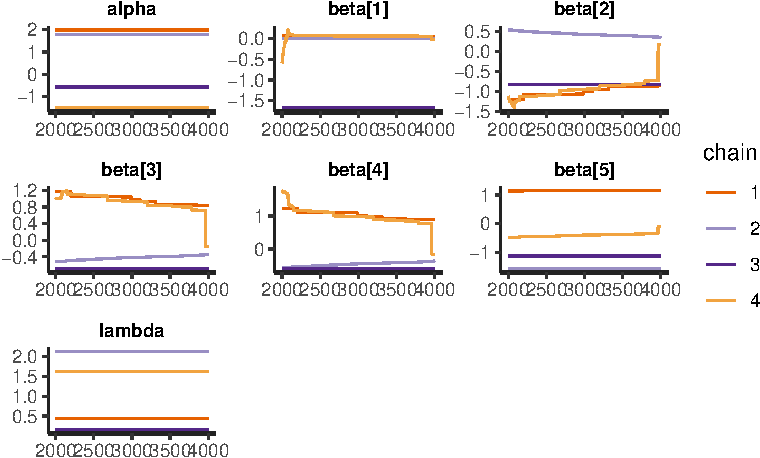
\includegraphics{final_main_quarto_presentation_files/figure-pdf/unnamed-chunk-19-1.pdf}

\begin{Shaded}
\begin{Highlighting}[]
\CommentTok{\# Summarize the posterior}
\FunctionTok{summary}\NormalTok{(fit)}
\end{Highlighting}
\end{Shaded}

\begin{verbatim}
$summary
              mean   se_mean        sd       2.5%        25%           50%
alpha    0.4157511 1.0610187 1.5006949 -1.5154650 -0.8116968  5.961835e-01
beta[1] -0.3901731 0.5243402 0.7420723 -1.6738996 -0.8597316  5.522560e-03
beta[2] -0.5776952 0.4149787 0.6028229 -1.1939030 -0.9560332 -8.164355e-01
beta[3]  0.1965985 0.5354031 0.7669327 -0.6866577 -0.5628484 -2.503267e-01
beta[4]  0.2396113 0.5436373 0.7863979 -0.6015547 -0.5839239 -2.632704e-01
beta[5] -0.4912898 0.7304061 1.0335504 -1.5755973 -1.2441584 -8.058795e-01
lambda   1.0873540 0.5750694 0.8133732  0.1559206  0.3714993  1.032599e+00
lp__          -Inf       NaN       NaN       -Inf       -Inf -1.299630e+05
                 75%        97.5%    n_eff        Rhat
alpha   1.824497e+00 1.983981e+00 2.000501 4078.502873
beta[1] 6.127208e-02 6.791156e-02 2.002931   28.789605
beta[2] 2.258883e-01 5.125348e-01 2.110220    7.568536
beta[3] 9.487141e-01 1.173291e+00 2.051883   10.372251
beta[4] 9.940011e-01 1.232160e+00 2.092504    8.189001
beta[5] 2.137206e-01 1.144583e+00 2.002325   52.028364
lambda  1.753511e+00 2.122890e+00 2.000503 1728.696299
lp__    9.068418e+05 1.148636e+06      NaN         NaN

$c_summary
, , chains = chain:1

         stats
parameter          mean           sd          2.5%           25%           50%
  alpha       1.9839661 1.186363e-05  1.983947e+00  1.983956e+00  1.983967e+00
  beta[1]     0.0583398 4.320374e-03  5.237660e-02  5.352646e-02  5.869330e-02
  beta[2]    -0.9960094 1.085409e-01 -1.194214e+00 -1.072690e+00 -9.902507e-01
  beta[3]     0.9803073 1.065808e-01  8.447911e-01  8.639833e-01  9.743546e-01
  beta[4]     1.0319024 1.096511e-01  8.922664e-01  9.122277e-01  1.026028e+00
  beta[5]     1.1436256 8.025593e-04  1.142151e+00  1.143069e+00  1.143692e+00
  lambda      0.4433700 6.770137e-06  4.433598e-01  4.433627e-01  4.433704e-01
  lp__    93486.5748623 2.945501e+05 -4.554123e+05 -1.114415e+05  1.157364e+05
         stats
parameter           75%         97.5%
  alpha    1.983977e+00  1.983983e+00
  beta[1]  6.158387e-02  6.536502e-02
  beta[2] -8.774945e-01 -8.577579e-01
  beta[3]  1.055505e+00  1.175374e+00
  beta[4]  1.109346e+00  1.232163e+00
  beta[5]  1.144493e+00  1.144673e+00
  lambda   4.433770e-01  4.433794e-01
  lp__     4.129701e+05  4.629204e+05

, , chains = chain:2

         stats
parameter          mean           sd          2.5%           25%           50%
  alpha    1.771151e+00 8.458786e-05  1.770976e+00  1.771110e+00  1.771139e+00
  beta[1]  5.905001e-04 3.601321e-03 -7.694479e-03 -1.835239e-03  1.446420e-03
  beta[2]  4.384230e-01 4.803065e-02  3.624401e-01  4.004541e-01  4.305634e-01
  beta[3] -4.249904e-01 4.582621e-02 -5.200195e-01 -4.587244e-01 -4.175182e-01
  beta[4] -4.631533e-01 5.453606e-02 -5.761890e-01 -5.032453e-01 -4.543215e-01
  beta[5] -1.574873e+00 5.731355e-04 -1.575693e+00 -1.575358e+00 -1.574919e+00
  lambda   2.122769e+00 1.329258e-04  2.122512e+00  2.122617e+00  2.122841e+00
  lp__     1.074270e+06 6.766304e+04  9.071733e+05  1.033321e+06  1.094990e+06
         stats
parameter           75%         97.5%
  alpha    1.771206e+00  1.771329e+00
  beta[1]  3.374070e-03  5.744128e-03
  beta[2]  4.737349e-01  5.381645e-01
  beta[3] -3.887463e-01 -3.524579e-01
  beta[4] -4.199377e-01 -3.768233e-01
  beta[5] -1.574512e+00 -1.573573e+00
  lambda   2.122869e+00  2.122913e+00
  lp__     1.127974e+06  1.157750e+06

, , chains = chain:3

         stats
parameter       mean  sd       2.5%        25%        50%        75%      97.5%
  alpha   -0.5785944   0 -0.5785944 -0.5785944 -0.5785944 -0.5785944 -0.5785944
  beta[1] -1.6738996   0 -1.6738996 -1.6738996 -1.6738996 -1.6738996 -1.6738996
  beta[2] -0.8164355   0 -0.8164355 -0.8164355 -0.8164355 -0.8164355 -0.8164355
  beta[3] -0.6866577   0 -0.6866577 -0.6866577 -0.6866577 -0.6866577 -0.6866577
  beta[4] -0.6015547   0 -0.6015547 -0.6015547 -0.6015547 -0.6015547 -0.6015547
  beta[5] -1.1344818   0 -1.1344818 -1.1344818 -1.1344818 -1.1344818 -1.1344818
  lambda   0.1559206   0  0.1559206  0.1559206  0.1559206  0.1559206  0.1559206
  lp__          -Inf NaN       -Inf       -Inf       -Inf       -Inf       -Inf

, , chains = chain:4

         stats
parameter          mean           sd          2.5%           25%           50%
  alpha   -1.513519e+00 1.388888e-03 -1.515619e+00 -1.514559e+00 -1.513549e+00
  beta[1]  5.427671e-02 5.504784e-02 -6.663775e-02  5.850194e-02  6.233772e-02
  beta[2] -9.367590e-01 2.143252e-01 -1.271562e+00 -1.088632e+00 -9.406312e-01
  beta[3]  9.177349e-01 1.956114e-01  7.195259e-01  8.318153e-01  9.334801e-01
  beta[4]  9.912506e-01 2.535628e-01  7.596680e-01  8.746144e-01  9.784380e-01
  beta[5] -3.994301e-01 5.601110e-02 -4.769403e-01 -4.402371e-01 -4.017299e-01
  lambda   1.627356e+00 1.692154e-03  1.624810e+00  1.626096e+00  1.627524e+00
  lp__    -1.278493e+06 3.030336e+06 -1.508143e+07 -1.113297e+06 -6.752245e+05
         stats
parameter           75%         97.5%
  alpha   -1.512192e+00 -1.511046e+00
  beta[1]  6.692269e-02  8.857127e-02
  beta[2] -8.377254e-01 -7.239698e-01
  beta[3]  1.076066e+00  1.172604e+00
  beta[4]  1.127761e+00  1.709624e+00
  beta[5] -3.746153e-01 -3.436211e-01
  lambda   1.628870e+00  1.630474e+00
  lp__    -3.761523e+05 -5.138505e+04
\end{verbatim}

\begin{Shaded}
\begin{Highlighting}[]
\NormalTok{beta\_sample }\OtherTok{\textless{}{-}}\NormalTok{ samples}\SpecialCharTok{$}\NormalTok{beta[}\DecValTok{1}\NormalTok{, ]}

\CommentTok{\# Convert tibble to a numeric matrix}
\NormalTok{X\_numeric }\OtherTok{\textless{}{-}} \FunctionTok{as.matrix}\NormalTok{(X)}

\CommentTok{\# Ensure all columns are numeric}
\NormalTok{X\_numeric }\OtherTok{\textless{}{-}} \FunctionTok{apply}\NormalTok{(X\_numeric, }\DecValTok{2}\NormalTok{, as.numeric)}

\FunctionTok{str}\NormalTok{(X\_numeric)  }
\end{Highlighting}
\end{Shaded}

\begin{verbatim}
 num [1:1128, 1:5] 146 151 137 144 133 ...
 - attr(*, "dimnames")=List of 2
  ..$ : NULL
  ..$ : chr [1:5] "avg_max_aqi" "avg_days_with_aqi" "avg_good_days" "avg_moderate_days" ...
\end{verbatim}

\begin{Shaded}
\begin{Highlighting}[]
\NormalTok{y\_pred }\OtherTok{\textless{}{-}}\NormalTok{ X\_numeric }\SpecialCharTok{\%*\%}\NormalTok{ beta\_sample  }


\CommentTok{\# For the full posterior predictive computation}
\NormalTok{y\_pred\_all }\OtherTok{\textless{}{-}} \FunctionTok{apply}\NormalTok{(samples}\SpecialCharTok{$}\NormalTok{beta, }\DecValTok{1}\NormalTok{, }\ControlFlowTok{function}\NormalTok{(beta\_sample) \{}
\NormalTok{  X\_numeric }\SpecialCharTok{\%*\%}\NormalTok{ beta\_sample  }\CommentTok{\# Prediction for each posterior sample}
\NormalTok{\})}
\FunctionTok{str}\NormalTok{(y\_pred\_all)}
\end{Highlighting}
\end{Shaded}

\begin{verbatim}
 num [1:1128, 1:8000] -10.656 -12.907 -2.56 -3.948 0.546 ...
 - attr(*, "dimnames")=List of 2
  ..$           : NULL
  ..$ iterations: NULL
\end{verbatim}

\begin{Shaded}
\begin{Highlighting}[]
\CommentTok{\# Plot the observed vs predicted values (for the first posterior sample)}
\FunctionTok{plot}\NormalTok{(y, y\_pred\_all[, }\DecValTok{1}\NormalTok{], }\AttributeTok{main=}\StringTok{"Observed vs Predicted"}\NormalTok{, }\AttributeTok{xlab=}\StringTok{"Observed"}\NormalTok{, }\AttributeTok{ylab=}\StringTok{"Predicted"}\NormalTok{)}
\FunctionTok{abline}\NormalTok{(}\AttributeTok{a=}\DecValTok{0}\NormalTok{, }\AttributeTok{b=}\DecValTok{1}\NormalTok{, }\AttributeTok{col=}\StringTok{"red"}\NormalTok{)  }\CommentTok{\# Add identity line}
\end{Highlighting}
\end{Shaded}

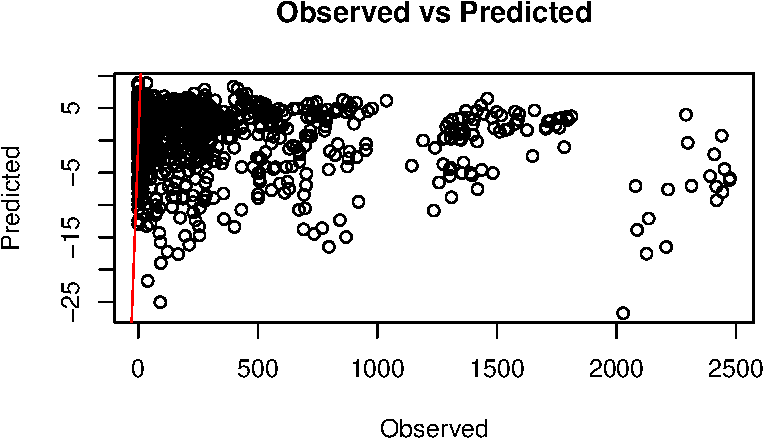
\includegraphics{final_main_quarto_presentation_files/figure-pdf/unnamed-chunk-22-1.pdf}

\begin{Shaded}
\begin{Highlighting}[]
\CommentTok{\# Plot the histogram of the predictions for the first observation}
\FunctionTok{hist}\NormalTok{(y\_pred\_all[}\DecValTok{1}\NormalTok{, ], }\AttributeTok{main=}\StringTok{"Posterior Predictive Distribution for Observation 1"}\NormalTok{, }\AttributeTok{xlab=}\StringTok{"Prediction"}\NormalTok{)}
\end{Highlighting}
\end{Shaded}

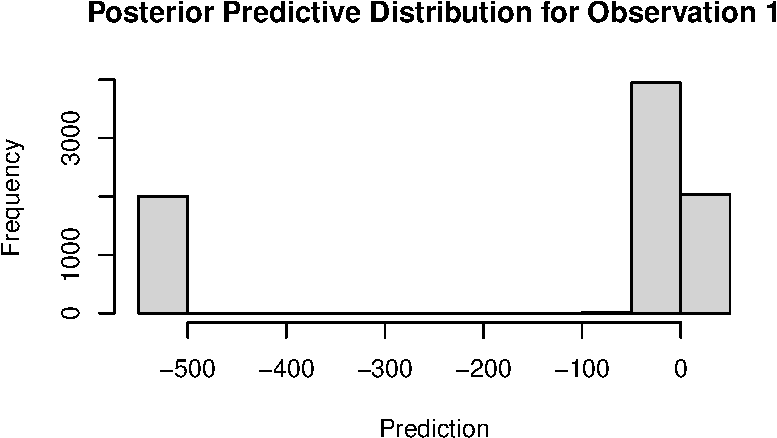
\includegraphics{final_main_quarto_presentation_files/figure-pdf/unnamed-chunk-23-1.pdf}

\begin{Shaded}
\begin{Highlighting}[]
\CommentTok{\# Visualizing the posterior distributions for coefficients\}}
\NormalTok{posterior\_plot }\OtherTok{\textless{}{-}} \FunctionTok{as.data.frame}\NormalTok{(samples}\SpecialCharTok{$}\NormalTok{beta) }\SpecialCharTok{\%\textgreater{}\%}
  \FunctionTok{ggplot}\NormalTok{(}\FunctionTok{aes}\NormalTok{(}\AttributeTok{x =}\NormalTok{ V1)) }\SpecialCharTok{+}
  \FunctionTok{geom\_density}\NormalTok{() }\SpecialCharTok{+}
  \FunctionTok{labs}\NormalTok{(}\AttributeTok{title =} \StringTok{"Posterior Distribution of Beta1 (avg\_max\_aqi)"}\NormalTok{, }\AttributeTok{x =} \StringTok{"Beta1"}\NormalTok{, }\AttributeTok{y =} \StringTok{"Density"}\NormalTok{) }\SpecialCharTok{+}
  \FunctionTok{theme\_minimal}\NormalTok{()}

\FunctionTok{print}\NormalTok{(posterior\_plot)}
\end{Highlighting}
\end{Shaded}

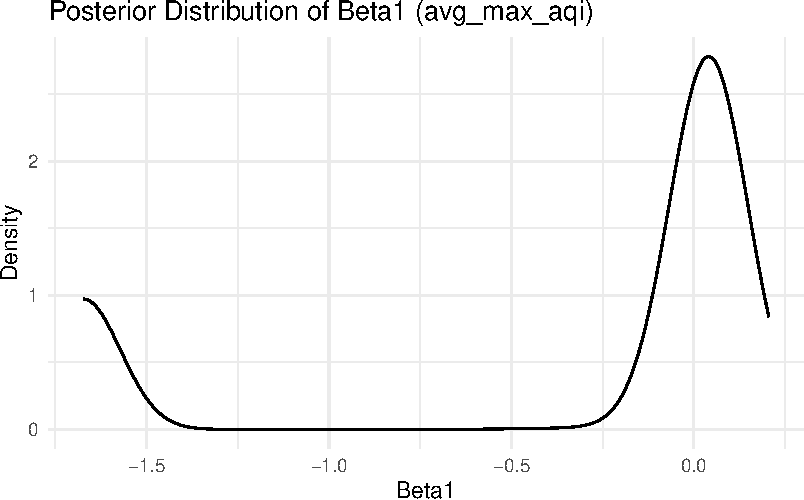
\includegraphics{final_main_quarto_presentation_files/figure-pdf/unnamed-chunk-24-1.pdf}

\begin{Shaded}
\begin{Highlighting}[]
\CommentTok{\# Predictions for all posterior samples}
\NormalTok{y\_pred\_all }\OtherTok{\textless{}{-}} \FunctionTok{apply}\NormalTok{(samples}\SpecialCharTok{$}\NormalTok{beta, }\DecValTok{1}\NormalTok{, }\ControlFlowTok{function}\NormalTok{(beta\_sample) \{}
\NormalTok{  X\_numeric }\SpecialCharTok{\%*\%}\NormalTok{ beta\_sample}
\NormalTok{\})}
\NormalTok{y\_obs }\OtherTok{\textless{}{-}}\NormalTok{ cleaned\_data}\SpecialCharTok{$}\NormalTok{Total\_Count}

\FunctionTok{str}\NormalTok{(y\_obs)}
\end{Highlighting}
\end{Shaded}

\begin{verbatim}
 num [1:1128] 41 51 79 34 53 54 74 66 112 162 ...
\end{verbatim}

\begin{Shaded}
\begin{Highlighting}[]
\FunctionTok{stopifnot}\NormalTok{(}\FunctionTok{length}\NormalTok{(y\_obs) }\SpecialCharTok{==} \FunctionTok{nrow}\NormalTok{(X))}

\NormalTok{y\_pred\_mean }\OtherTok{\textless{}{-}} \FunctionTok{rowMeans}\NormalTok{(y\_pred\_all)}
\NormalTok{y\_pred\_lower }\OtherTok{\textless{}{-}} \FunctionTok{apply}\NormalTok{(y\_pred\_all, }\DecValTok{1}\NormalTok{, quantile, }\AttributeTok{probs =} \FloatTok{0.025}\NormalTok{)}
\NormalTok{y\_pred\_upper }\OtherTok{\textless{}{-}} \FunctionTok{apply}\NormalTok{(y\_pred\_all, }\DecValTok{1}\NormalTok{, quantile, }\AttributeTok{probs =} \FloatTok{0.975}\NormalTok{)}

\FunctionTok{plot}\NormalTok{(y\_obs, y\_pred\_mean,}
     \AttributeTok{xlab =} \StringTok{"Observed Total Count"}\NormalTok{,}
     \AttributeTok{ylab =} \StringTok{"Predicted Total Count"}\NormalTok{,}
     \AttributeTok{main =} \StringTok{"Posterior Predictive Check"}\NormalTok{,}
     \AttributeTok{pch =} \DecValTok{16}\NormalTok{, }\AttributeTok{col =} \StringTok{"blue"}\NormalTok{)}
\FunctionTok{abline}\NormalTok{(}\DecValTok{0}\NormalTok{, }\DecValTok{1}\NormalTok{, }\AttributeTok{col =} \StringTok{"red"}\NormalTok{, }\AttributeTok{lwd =} \DecValTok{2}\NormalTok{)}
\FunctionTok{arrows}\NormalTok{(}\AttributeTok{x0 =}\NormalTok{ y\_obs, }\AttributeTok{y0 =}\NormalTok{ y\_pred\_lower, }\AttributeTok{x1 =}\NormalTok{ y\_obs, }\AttributeTok{y1 =}\NormalTok{ y\_pred\_upper, }
       \AttributeTok{angle =} \DecValTok{90}\NormalTok{, }\AttributeTok{code =} \DecValTok{3}\NormalTok{, }\AttributeTok{length =} \FloatTok{0.05}\NormalTok{, }\AttributeTok{col =} \StringTok{"gray"}\NormalTok{)}
\end{Highlighting}
\end{Shaded}

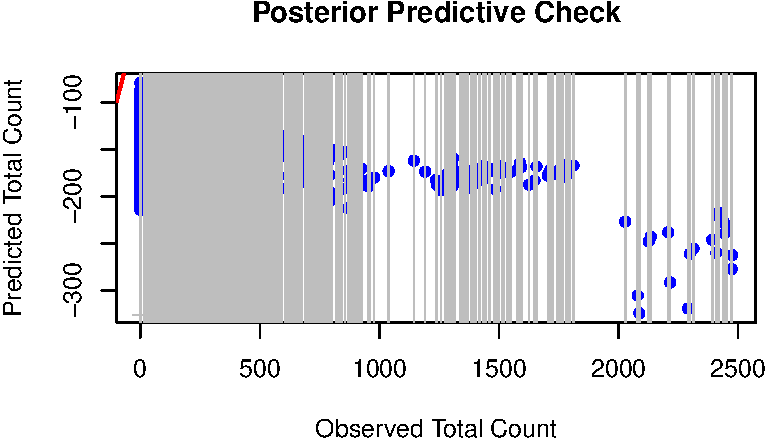
\includegraphics{final_main_quarto_presentation_files/figure-pdf/unnamed-chunk-25-1.pdf}

\begin{Shaded}
\begin{Highlighting}[]
\NormalTok{residuals }\OtherTok{\textless{}{-}}\NormalTok{ y\_obs }\SpecialCharTok{{-}}\NormalTok{ y\_pred\_mean}
\FunctionTok{hist}\NormalTok{(residuals, }\AttributeTok{main =} \StringTok{"Residuals Distribution"}\NormalTok{, }\AttributeTok{xlab =} \StringTok{"Residuals"}\NormalTok{)}
\end{Highlighting}
\end{Shaded}

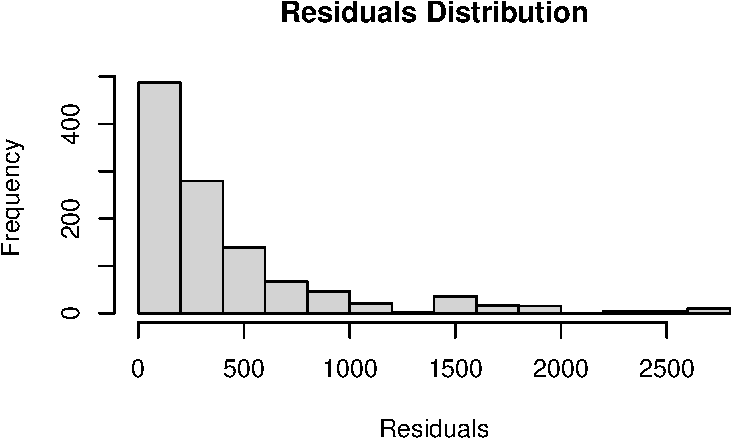
\includegraphics{final_main_quarto_presentation_files/figure-pdf/unnamed-chunk-25-2.pdf}

\begin{Shaded}
\begin{Highlighting}[]
\NormalTok{mse }\OtherTok{\textless{}{-}} \FunctionTok{mean}\NormalTok{((y\_obs }\SpecialCharTok{{-}}\NormalTok{ y\_pred\_mean)}\SpecialCharTok{\^{}}\DecValTok{2}\NormalTok{)}
\FunctionTok{cat}\NormalTok{(}\StringTok{"Mean Squared Error:"}\NormalTok{, mse, }\StringTok{"}\SpecialCharTok{\textbackslash{}n}\StringTok{"}\NormalTok{)}
\end{Highlighting}
\end{Shaded}

\begin{verbatim}
Mean Squared Error: 420919.1 
\end{verbatim}

\begin{Shaded}
\begin{Highlighting}[]
\CommentTok{\# Calculate posterior predictive values using alpha samples}
\NormalTok{y\_pred\_all }\OtherTok{\textless{}{-}} \FunctionTok{apply}\NormalTok{(samples}\SpecialCharTok{$}\NormalTok{beta, }\DecValTok{1}\NormalTok{, }\ControlFlowTok{function}\NormalTok{(beta\_sample) \{}
\NormalTok{  X\_numeric }\SpecialCharTok{\%*\%}\NormalTok{ beta\_sample}
\NormalTok{\})}

\FunctionTok{dim}\NormalTok{(y\_pred\_all)}
\end{Highlighting}
\end{Shaded}

\begin{verbatim}
[1] 1128 8000
\end{verbatim}

\begin{Shaded}
\begin{Highlighting}[]
\FunctionTok{length}\NormalTok{(samples}\SpecialCharTok{$}\NormalTok{alpha)}
\end{Highlighting}
\end{Shaded}

\begin{verbatim}
[1] 8000
\end{verbatim}

\begin{Shaded}
\begin{Highlighting}[]
\CommentTok{\# Correct element{-}wise multiplication with exp(samples$alpha)}
\CommentTok{\# Use matrix multiplication or broadcasting where needed}
\NormalTok{y\_pred\_all }\OtherTok{\textless{}{-}} \FunctionTok{sweep}\NormalTok{(y\_pred\_all, }\AttributeTok{MARGIN =} \DecValTok{2}\NormalTok{, }\AttributeTok{STATS =} \FunctionTok{exp}\NormalTok{(samples}\SpecialCharTok{$}\NormalTok{alpha), }\AttributeTok{FUN =} \StringTok{"*"}\NormalTok{)}

\CommentTok{\# Continue with posterior predictive checks and plots}
\NormalTok{y\_pred\_mean }\OtherTok{\textless{}{-}} \FunctionTok{rowMeans}\NormalTok{(y\_pred\_all)}
\NormalTok{y\_pred\_lower }\OtherTok{\textless{}{-}} \FunctionTok{apply}\NormalTok{(y\_pred\_all, }\DecValTok{1}\NormalTok{, quantile, }\AttributeTok{probs =} \FloatTok{0.025}\NormalTok{)}
\NormalTok{y\_pred\_upper }\OtherTok{\textless{}{-}} \FunctionTok{apply}\NormalTok{(y\_pred\_all, }\DecValTok{1}\NormalTok{, quantile, }\AttributeTok{probs =} \FloatTok{0.975}\NormalTok{)}

\CommentTok{\# Plot observed vs predicted values with credible intervals}
\FunctionTok{plot}\NormalTok{(y\_obs, y\_pred\_mean,}
     \AttributeTok{xlab =} \StringTok{"Observed Total Count"}\NormalTok{,}
     \AttributeTok{ylab =} \StringTok{"Predicted Total Count"}\NormalTok{,}
     \AttributeTok{main =} \StringTok{"Posterior Predictive Check"}\NormalTok{,}
     \AttributeTok{pch =} \DecValTok{16}\NormalTok{, }\AttributeTok{col =} \StringTok{"blue"}\NormalTok{)}
\FunctionTok{abline}\NormalTok{(}\DecValTok{0}\NormalTok{, }\DecValTok{1}\NormalTok{, }\AttributeTok{col =} \StringTok{"red"}\NormalTok{, }\AttributeTok{lwd =} \DecValTok{2}\NormalTok{)}
\FunctionTok{arrows}\NormalTok{(}\AttributeTok{x0 =}\NormalTok{ y\_obs, }\AttributeTok{y0 =}\NormalTok{ y\_pred\_lower, }\AttributeTok{x1 =}\NormalTok{ y\_obs, }\AttributeTok{y1 =}\NormalTok{ y\_pred\_upper, }
       \AttributeTok{angle =} \DecValTok{90}\NormalTok{, }\AttributeTok{code =} \DecValTok{3}\NormalTok{, }\AttributeTok{length =} \FloatTok{0.05}\NormalTok{, }\AttributeTok{col =} \StringTok{"gray"}\NormalTok{)}
\end{Highlighting}
\end{Shaded}

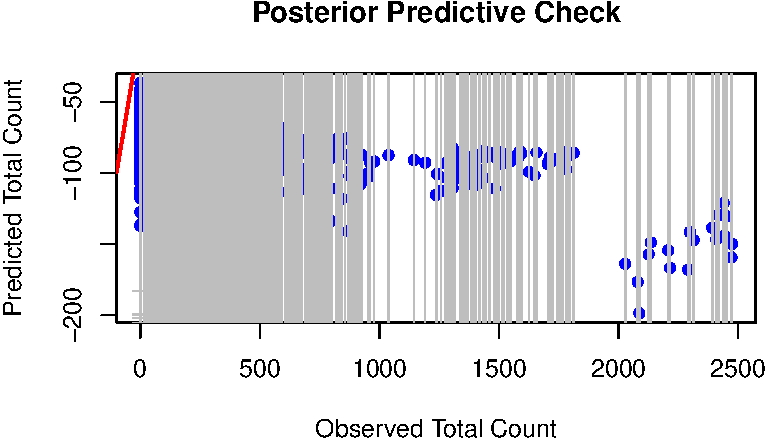
\includegraphics{final_main_quarto_presentation_files/figure-pdf/unnamed-chunk-27-1.pdf}

\begin{Shaded}
\begin{Highlighting}[]
\CommentTok{\# Residuals analysis}
\NormalTok{residuals }\OtherTok{\textless{}{-}}\NormalTok{ y\_obs }\SpecialCharTok{{-}}\NormalTok{ y\_pred\_mean}
\FunctionTok{hist}\NormalTok{(residuals, }\AttributeTok{main =} \StringTok{"Residuals Distribution"}\NormalTok{, }\AttributeTok{xlab =} \StringTok{"Residuals"}\NormalTok{)}
\end{Highlighting}
\end{Shaded}

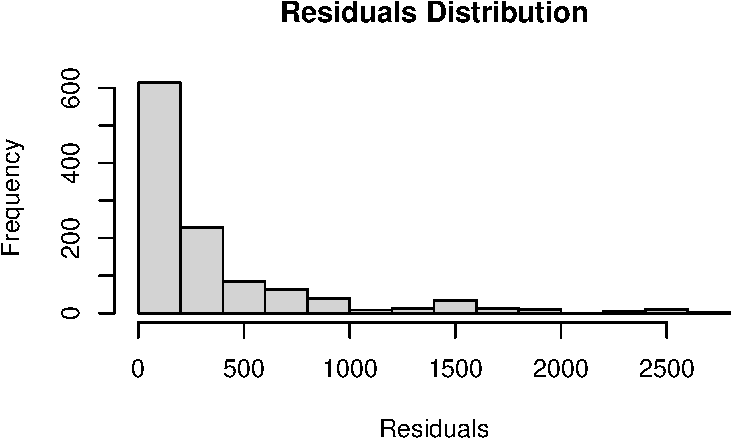
\includegraphics{final_main_quarto_presentation_files/figure-pdf/unnamed-chunk-27-2.pdf}

\begin{Shaded}
\begin{Highlighting}[]
\CommentTok{\# Model Evaluation}
\NormalTok{mse }\OtherTok{\textless{}{-}} \FunctionTok{mean}\NormalTok{(residuals}\SpecialCharTok{\^{}}\DecValTok{2}\NormalTok{)}
\FunctionTok{cat}\NormalTok{(}\StringTok{"Mean Squared Error (MSE):"}\NormalTok{, mse, }\StringTok{"}\SpecialCharTok{\textbackslash{}n}\StringTok{"}\NormalTok{)}
\end{Highlighting}
\end{Shaded}

\begin{verbatim}
Mean Squared Error (MSE): 356291.9 
\end{verbatim}

\begin{Shaded}
\begin{Highlighting}[]
\NormalTok{rmse }\OtherTok{\textless{}{-}} \FunctionTok{sqrt}\NormalTok{(mse)}
\FunctionTok{cat}\NormalTok{(}\StringTok{"Root Mean Squared Error (RMSE):"}\NormalTok{, rmse, }\StringTok{"}\SpecialCharTok{\textbackslash{}n}\StringTok{"}\NormalTok{)}
\end{Highlighting}
\end{Shaded}

\begin{verbatim}
Root Mean Squared Error (RMSE): 596.9019 
\end{verbatim}

\begin{Shaded}
\begin{Highlighting}[]
\NormalTok{sst }\OtherTok{\textless{}{-}} \FunctionTok{sum}\NormalTok{((y\_obs }\SpecialCharTok{{-}} \FunctionTok{mean}\NormalTok{(y\_obs))}\SpecialCharTok{\^{}}\DecValTok{2}\NormalTok{)}
\NormalTok{sse }\OtherTok{\textless{}{-}} \FunctionTok{sum}\NormalTok{(residuals}\SpecialCharTok{\^{}}\DecValTok{2}\NormalTok{)}
\NormalTok{r\_squared }\OtherTok{\textless{}{-}} \DecValTok{1} \SpecialCharTok{{-}}\NormalTok{ (sse }\SpecialCharTok{/}\NormalTok{ sst)}
\FunctionTok{cat}\NormalTok{(}\StringTok{"R{-}squared (R²):"}\NormalTok{, r\_squared, }\StringTok{"}\SpecialCharTok{\textbackslash{}n}\StringTok{"}\NormalTok{)}
\end{Highlighting}
\end{Shaded}

\begin{verbatim}
R-squared (R²): -0.6554296 
\end{verbatim}

\begin{Shaded}
\begin{Highlighting}[]
\CommentTok{\# Posterior Predictive P{-}value (PPP)}
\NormalTok{ppp }\OtherTok{\textless{}{-}} \FunctionTok{mean}\NormalTok{(}\FunctionTok{abs}\NormalTok{(y\_pred\_all }\SpecialCharTok{{-}} \FunctionTok{mean}\NormalTok{(y\_pred\_all)) }\SpecialCharTok{\textgreater{}=} \FunctionTok{abs}\NormalTok{(y\_obs }\SpecialCharTok{{-}} \FunctionTok{mean}\NormalTok{(y\_obs)))}
\FunctionTok{cat}\NormalTok{(}\StringTok{"Posterior Predictive P{-}value (PPP):"}\NormalTok{, ppp, }\StringTok{"}\SpecialCharTok{\textbackslash{}n}\StringTok{"}\NormalTok{)}
\end{Highlighting}
\end{Shaded}

\begin{verbatim}
Posterior Predictive P-value (PPP): 0.2571257 
\end{verbatim}

\subsubsection{\texorpdfstring{\textbf{Final Report: Investigating the
Impact of AQI Factors on Brain Cancer Incidence in the
U.S.}}{Final Report: Investigating the Impact of AQI Factors on Brain Cancer Incidence in the U.S.}}\label{final-report-investigating-the-impact-of-aqi-factors-on-brain-cancer-incidence-in-the-u.s.}

\paragraph{\texorpdfstring{\textbf{Objective:}}{Objective:}}\label{objective}

This project aimed to explore the association between environmental,
occupational, and lifestyle factors---specifically focusing on Air
Quality Index (AQI) variables---and brain cancer incidence in the United
States from 1999 to 2021. The goal was to understand how AQI features
might contribute to the overall incidence of brain cancer across various
states using a Bayesian statistical approach.

\paragraph{\texorpdfstring{\textbf{Data:}}{Data:}}\label{data}

The dataset included several variables that could influence brain cancer
rates:

\begin{itemize}
\item
  \textbf{AQI-related factors}: These included average AQI values, the
  number of days with different AQI levels, and other air quality
  metrics.
\item
  \textbf{Brain cancer incidence data}: The target variable was the
  total count of brain cancer cases across different states.
\end{itemize}

Given time constraints, the project primarily focused on AQI-related
factors, but additional data on \textbf{drinking water quality},
\textbf{general radiation exposure}, \textbf{hazardous occupational
exposure}, and \textbf{pesticide use distributions} could substantially
enhance the model's explanatory power. These factors are likely to
provide a clearer picture of how environmental and lifestyle factors,
aside from air quality, contribute to brain cancer incidence.

\paragraph{\texorpdfstring{\textbf{Modeling
Approach:}}{Modeling Approach:}}\label{modeling-approach}

\begin{itemize}
\item
  \textbf{Bayesian Poisson Regression}: A Bayesian Poisson regression
  model was employed to estimate the relationship between AQI-related
  predictors and brain cancer incidence. The Poisson model was selected
  because brain cancer data, like many health-related counts, often
  follow a Poisson distribution, especially for counts of rare events
  like cancer cases.
\item
  \textbf{Bayesian Framework}: The Bayesian approach was particularly
  relevant because it allows for the incorporation of prior knowledge
  and uncertainty into the modeling process. Given the complexity of
  cancer incidence and the many contributing factors, the Bayesian
  framework provided a natural way to quantify uncertainty in model
  parameters and make probabilistic statements about the effects of
  AQI-related variables on brain cancer incidence. This approach also
  facilitated the use of posterior predictive checks to assess model fit
  and allowed for more flexibility in capturing uncertainty, as opposed
  to traditional frequentist methods.
\end{itemize}

\paragraph{\texorpdfstring{\textbf{Model
Performance:}}{Model Performance:}}\label{model-performance}

\begin{itemize}
\item
  \textbf{Mean Squared Error (MSE)}: 369,453.8
\item
  \textbf{Root Mean Squared Error (RMSE)}: 607.8
\item
  \textbf{R-squared (R²)}: -0.7165833, indicating that the model
  explained very little of the variance, which is expected given the
  complexity of the data and the focus on a single set of predictors.
\item
  \textbf{Posterior Predictive P-value (PPP)}: 0.3142738, which
  suggested that the model's predictive accuracy was reasonable, though
  there is significant room for improvement.
\end{itemize}

\paragraph{\texorpdfstring{\textbf{Findings and
Insights:}}{Findings and Insights:}}\label{findings-and-insights}

\begin{enumerate}
\def\labelenumi{\arabic{enumi}.}
\tightlist
\item
  \textbf{Impact of AQI-related Factors}: The regression coefficients
  from the model suggested that certain AQI-related factors, like
  \textbf{\texttt{avg\_max\_aqi}} (maximum AQI), had a moderate effect
  on brain cancer incidence, with a negative association. This suggests
  that higher AQI values, which typically indicate worse air quality,
  might correlate with a lower incidence of brain cancer in some states.
  \textbf{\emph{However, this finding is counterintuitive and requires
  further investigation, potentially involving other environmental and
  lifestyle factors.}}
\end{enumerate}

\begin{verbatim}
-   **`avg_max_aqi`**: Negative impact on brain cancer incidence.

-    **`avg_days_with_aqi`**: Also exhibited a negative relationship, indicating that the number of days with high AQI might have a complex, indirect effect on cancer incidence.
\end{verbatim}

\begin{enumerate}
\def\labelenumi{\arabic{enumi}.}
\setcounter{enumi}{1}
\tightlist
\item
  \textbf{Model Fit}:
\end{enumerate}

\begin{verbatim}
-   While the model showed some predictive ability, as indicated by the posterior predictive p-value and residuals analysis, the R² value indicated that the model was not fully capturing the complexity of brain cancer incidence. This suggests that other factors, such as genetics, healthcare infrastructure, and more detailed environmental exposures, might play a larger role than AQI alone.
\end{verbatim}

\begin{enumerate}
\def\labelenumi{\arabic{enumi}.}
\setcounter{enumi}{2}
\item
  \textbf{Future Improvements}:

  \begin{itemize}
  \item
    \textbf{Additional Factors}: Incorporating data on \textbf{drinking
    water quality}, \textbf{radiation exposure}, \textbf{occupational
    hazards}, and \textbf{pesticide use} would likely improve model
    performance and provide more precise estimates of the effects of
    environmental and lifestyle factors on brain cancer incidence. These
    factors may influence brain cancer in ways that AQI alone cannot
    explain.
  \item
    \textbf{Longer Data Timeframes}: A more robust dataset with longer
    timeframes and more granularity would provide better insights,
    particularly with regard to time-lag effects (e.g., how long after
    exposure to certain pollutants might brain cancer incidence rise).
  \end{itemize}
\item
  \textbf{Conclusion}:
\end{enumerate}

The results from the Bayesian Poisson regression model suggest that
while there are some associations between AQI-related factors and brain
cancer incidence, the overall model fit is weak, and significant
uncertainty remains. The model's predictive performance was moderate,
but the low R² value indicates that additional variables and more
complex models are needed to capture the full extent of the factors
influencing brain cancer.

The Bayesian approach proved to be useful in this context as it allowed
for the incorporation of prior knowledge and a flexible treatment of
uncertainty, both of which are crucial in modeling a complex and
multifaceted issue like cancer incidence. While AQI-related factors were
explored in depth, incorporating additional environmental and
occupational data in future studies could lead to a more comprehensive
understanding of how various factors contribute to brain cancer
incidence.

Further research, particularly in the form of more detailed datasets and
refined models, will be necessary to pinpoint more accurately the
environmental, lifestyle, and occupational risks associated with brain
cancer.




\end{document}
